\chapter{Gaussian random field generators for simulating partially coherent radiation}
\label{Chapter:Gaussian random field generators for simulating partially coherent radiation}
%\label{Chapter:White noise based algorithms for modeling Gaussian random processes}

    \rr{Say more about advantages and disadvantages of SERVAL to better show the difference between the common methods and SERVAL}  

    Radiation sources typically comprise numerous emitters contributing to the emission process. As the number of emitters becomes exceedingly large, it becomes impractical to describe these sources deterministically, leading to their characterization as random sources. In such scenarios, the theory of statistical optics offers an ideal framework for describing the behavior of electromagnetic fields emitted by these sources. Examples of random sources include thermal sources like stars and light bulbs, as well as radiation from ultra-relativistic particle bunches, such as synchrotron radiation and self-amplified spontaneous emission (SASE) free-electron laser (FEL) radiation in the linear regime. A common feature among these sources is their adherence to Gaussian statistics. According to the central limit theorem, as the number of random emitters increases, the resulting radiation, regardless of the probabilistic laws governing individual emitters, tends to follow a Gaussian statistics.

    \rr{finalise this…}  
    There are several methods for simulating statistical optics phenomena and the most frequently applied in the synchrotron radiation and FEL communities are mode decomposition methods~\rr{cite} and Monte-Carlo-based simulations, where radiation from each particle is simulated separately~\cite{chubar_accurate_1998, reiche_genesis_1999}. … 

    In this chapter, I present a set of methods for simulating Gaussian random fields based on a computationally efficient algorithm that leverages the properties of Gaussian random noise. This algorithm shapes the field distribution by multiplying the noise distribution with specifically chosen mathematical supports. These methods are designed exclusively for Gaussian random fields. However, there is potential to extend these methods to non-Gaussian statistics, as demonstrated in~\cite{hong_algorithm_2021}. Although these algorithms were developed for simulating synchrotron radiation (SR) sources and self-amplified spontaneous emission (SASE) free-electron laser (FEL) radiation, they can be easily extended to all optical fields that are stochastic and follow Gaussian statistics.
   
    These methods necessitate an introduction to the fundamentals of statistical optics theory, which I present earlier in this chapter. I begin with general definitions of random processes and their properties. Delving into the concepts of stationarity and ergodicity, I discuss differences in averaging processes: over time versus across different statistical realizations. Then, I introduce the central theoretical concept for this thesis—Gaussian random processes. Subsequently, I present the theory for quasi-stationary sources in a manner similar to that used in~\cite{mandel_optical_1995, goodman_statistical_2015} for stationary sources. I provide a proof of a generalized form of the Wiener-Khinchin theorem. This generalization accounts for the quasi-stationarity of a source and relates the finite duration of the pulse to spectral coherence properties. From the longitudinal coherence properties of radiation, I transition to the transverse domain of radiation and offer a derivation of the generalized van Cittert-Zernike theorem. Following this, I discuss the coherence properties of synchrotron and SASE FEL radiation, along with well-established methods for simulating these types of radiation sources. To this end, I introduce white-noise-based methods for simulating partially coherent radiation. Each method is first presented through heuristic considerations, which are then extended to applications in simulation problems: bending magnet radiation, undulator radiation, and FEL SASE radiation, as represented in Papers I, II, and III. Finalizing this chapter, I present an experimental method for generating sub-femtosecond level pulses at FEL facilities. The statistics of the pulses deviate from Gaussian behavior. This result showcases that the proposed algorithms should be applied carefully to the studied case when attempting to replicate the results in simulations.

\section{Classification of random processes}

    \rr{Say that the narrative here is shorten to the bare minimum needed for this thesis, and surely one can find more detail in~\cite{mandel_optical_1995, goodman_statistical_2015}. Also it should be noted separately, that I introduce theory for quasi-stationary sources, which is not presented in the textbooks}
    
    In this section, I will introduce the basic notations and concepts of statistical optics. I primarily follow the textbooks~\cite{mandel_optical_1995, goodman_statistical_2015} with slight modifications to encompass quasi-stationary sources in the theory. I start by introducing a random process $U$. This process consists of statistical realizations, which I denote as $u^{[k]}$. Unlike a random variable, such as a single roll of a dice, a random process also depends on time, represented as $u^{[k]}(t)$. Realistically, an observer can observe this process over a finite time interval $[-T/2, T/2]$. The process is random, meaning that the exact value of a given statistical realization $u^{[k]}(t_0)$ at a specific moment in time $t_0$ cannot be predicted in advance. One objective way to make predictions about a statistical process is to define statistical moments, which can be defined as follows:
    \begin{align}
        \overline{u(t)} = \frac{1}{T} \int \limits_{t - T/2}^{t + T/2}  u^{[k]}(t') dt',
        \label{Eq:time_avr}
    \end{align}
    and for the second moment or \textit{time auto-correlation function} I write:
    \begin{align}
        \overline{u(t_1)u(t_2)} = \frac{1}{T} \int \limits_{t - T/2}^{t + T/2} u^{[k]}(t + t_1)u^{[k]}(t + t_2)dt.
        \label{Eq:time_autocorrelation}
    \end{align}
    \rr{…and conclude…}
    
    For each process, I can define a set of probability density functions $p(u, t_i)$, which depend on both time and the chosen realization. To fully describe a statistical process, one needs to know not only $p(u, t_i)$—the first-order probability density function—but also its higher-order counterparts that contain information about correlations at different moments in time: $t_1, t_2, \ldots, t_n$, where, in principle, $n$ should be infinite. Therefore, one needs to know the second-order moment $p_2(u_1, t_1, u_2, t_2)$, the third, and up to the $n$-th order joint probability density function $p_n(u_1, t_1, u_2, t_2, \ldots, u_n, t_n)$. \rr{…again need to be concluded…} To anticipate, in the next chapter, I will introduce a type of process called Gaussian, where the process can be fully defined only by knowing the first and second-order probability density functions. With probability density functions I can define the ensemble averaging operation:
    \begin{align}
        \langle u(t) \rangle = \int u p(u, t) du,
        \label{Eq:ensemble_int_avr}
    \end{align}
    and similarly for the second order:
    \begin{align}
        \Gamma(t_1, t_2) = \langle u(t_1)u(t_2) \rangle = \iint u_1u_2 p_2(u_1, t_1, u_2, t_2) du_1du_2,
        \label{Eq:ensemble_int_autocorrelation}
    \end{align}
    and so on for higher order correlation functions. In principle, to fully describe a process, one needs to know all higher-order auto-correlation functions. However, in practice, it is often not possible to know all joint probability functions. In this case, one can utilize another useful definition of the ensemble averaging. If one collects a reasonably large statistical ensemble: $u^{[1]}(t), u^{[2]}(t), \ldots, u^{[k]}(t)$, then the ensemble average can be defined as averaging over the realisations:
    \begin{align}
        \langle u(t) \rangle = \lim_{N\to\infty} \frac{1}{N}\sum_{i=1}^{N} u^{[i]}(t)
        \label{Eq:ensemble_avr}
    \end{align}
    and the same for the second order auto-correlation function:
    \begin{align}
        \Gamma(t_1, t_2) = \langle u(t_1)u(t_2) \rangle = \lim_{N\to\infty} \frac{1}{N}\sum_{i=1}^{N} u^{[i]}(t_1)u^{[i]}(t_2),
        \label{Eq:ensemble_autocorrelation}
    \end{align}
    and so on for higher-order correlation functions. These definitions are fully equivalent to Eq.~\ref{Eq:ensemble_int_avr},~\ref{Eq:ensemble_int_autocorrelation}but are much more useful in practice. They only require measurement of the realizations themselves without any \textit{a priori} knowledge about the process. In this thesis, I will mostly rely on these latter definitions for practical calculations and the experiments.
    
    \subsection{Stationarity and ergodicity}
    
    Continuing the discussion about random processes, it is essential to identify properties that classify these processes and establish governing laws. In this subsection, I will introduce two important concepts in statistical optics: stationarity and ergodicity. These concepts classify processes based on their temporal characteristics and link these characteristics to their statistical realizations.

    I can define a requirement for a process to be stationary if all its joint probability density functions has the following property:
    \begin{align}
        p_n(u_1, t_1, u_2, t_2, …u_n, t_n) = p_n(u_1, t_1 + T, u_2, t_2 + T, …u_n, t_n + T) \; \textup{for all} \; T
        \label{Eq:stationary_strict}
    \end{align}
    As the choice of $T$ is arbitrary, we can set it to be one of the $t_n$ variables and find that, for example, the autocorrelation function depends only on the time difference $\Delta t = t_2 - t_1$.
    \begin{align}
        \Gamma(t_1, t_2) = \lim_{N\to\infty} \frac{1}{N}\sum_{i=1}^{N} u^{[i]}(t)u^{[i]}(t + t_2 - t_1) = \langle u(t)u(t + t_2 - t_1) \rangle
    \end{align}
    for all $t$ values.

    
    The definition in Eq.~\ref{Eq:stationary_strict} is also called \textit{strict-sense stationarity} because it requires that all orders of the joint probability function follow that definition. In practice, when one is interested only in the average and the first-order correlation function, a weaker definition can be used. If these two quantities are stationary, the process is called \textit{wide-sense stationarity}.

    As one can see, there are two conceptual ways to define averages in statistical optics: \textit{over} time and \textit{across} different realizations. In general, these averages should be different, but there is a specific type of process for which these two averages are equivalent. This type of process is called \textit{ergodic}. Writing the definition for this explicitly:
    \begin{align}
        \lim_{N\to\infty} \frac{1}{N}\sum_{i=1}^{N} u^{[i]}(t) = \frac{1}{T} \int \limits_{t - T/2}^{t + T/2}  u^{[k]}(t') dt'
    \end{align} 
    for any $t$, $T$ and taken $k$-th realization of the process. And the same can be written for the autocorrelation function:
    \begin{align}
        \lim_{N\to\infty} \frac{1}{N}\sum_{i=1}^{N} u^{[i]}(t_1)u^{[i]}(t_2) = \frac{1}{T} \int \limits_{t - T/2}^{t + T/2} u^{[k]}(t + t_1)u^{[k]}(t + t_2)dt
        \label{Eq:ergodic_corr}
    \end{align}
    again for any $t$, $T$ and taken $k$-th realization. \rr{…probably I am missing something here…}

    To state that a process is ergodic, one must verify similar equalities for all higher-order correlation functions of the process. However, there is a specific type of process called a Gaussian random process \r{I use in thesis terms Gaussian process, Gaussian statistics etc, and need to have some kind of disclaimer and/or boil them down to some system}, where once the first-order correlation function is known, all higher-order correlations can be expressed through it. In this case, if the process adheres to the definition in Eq.~\ref{Eq:ergodic_corr} then the process is strictly ergodic, and all higher-order correlation functions will satisfy similar equalities to Eq.~\ref{Eq:ergodic_corr}.

    \subsection{Gaussian random processes}
    \label{Sec:Gaussian random processes}
    Gaussian random processes play a pivotal role in statistical optics. Expressing this kind of statistics in mathematical terms, I start with the definition for the probability density function for a random process $x$:
    \begin{align}
        p(x) = \cfrac{1}{\sqrt{2 \pi}\sigma} e^{-x^2/2\sigma^2},
    \end{align}
    \rr{…check math…}
    where $\sigma$ is the dispersion of a random process $x$. It is always convenient to work with an analytic representation of a signal, so I introduce here a definition of the complex Gaussian random processes: $z = x + iy$, where both processes $x$ and $y$ have the same value of dispersion.
    \begin{align}
        p(z) = p(x)p(y) = \cfrac{1}{\sqrt{2 \pi}\sigma} e^{-(x^2 + y^2)/2\sigma^2},
    \end{align}
    which can be transformed using polar coordinates $x = A\cos(\phi)$ and $y = A\sin(\phi)$ to the following:
    \begin{align}
        p(z) = p(A, \phi) = \cfrac{A}{\sqrt{2 \pi}\sigma} e^{-A^2/2\sigma^2}.
    \end{align}
    \begin{figure}[h!]
    	\centering
        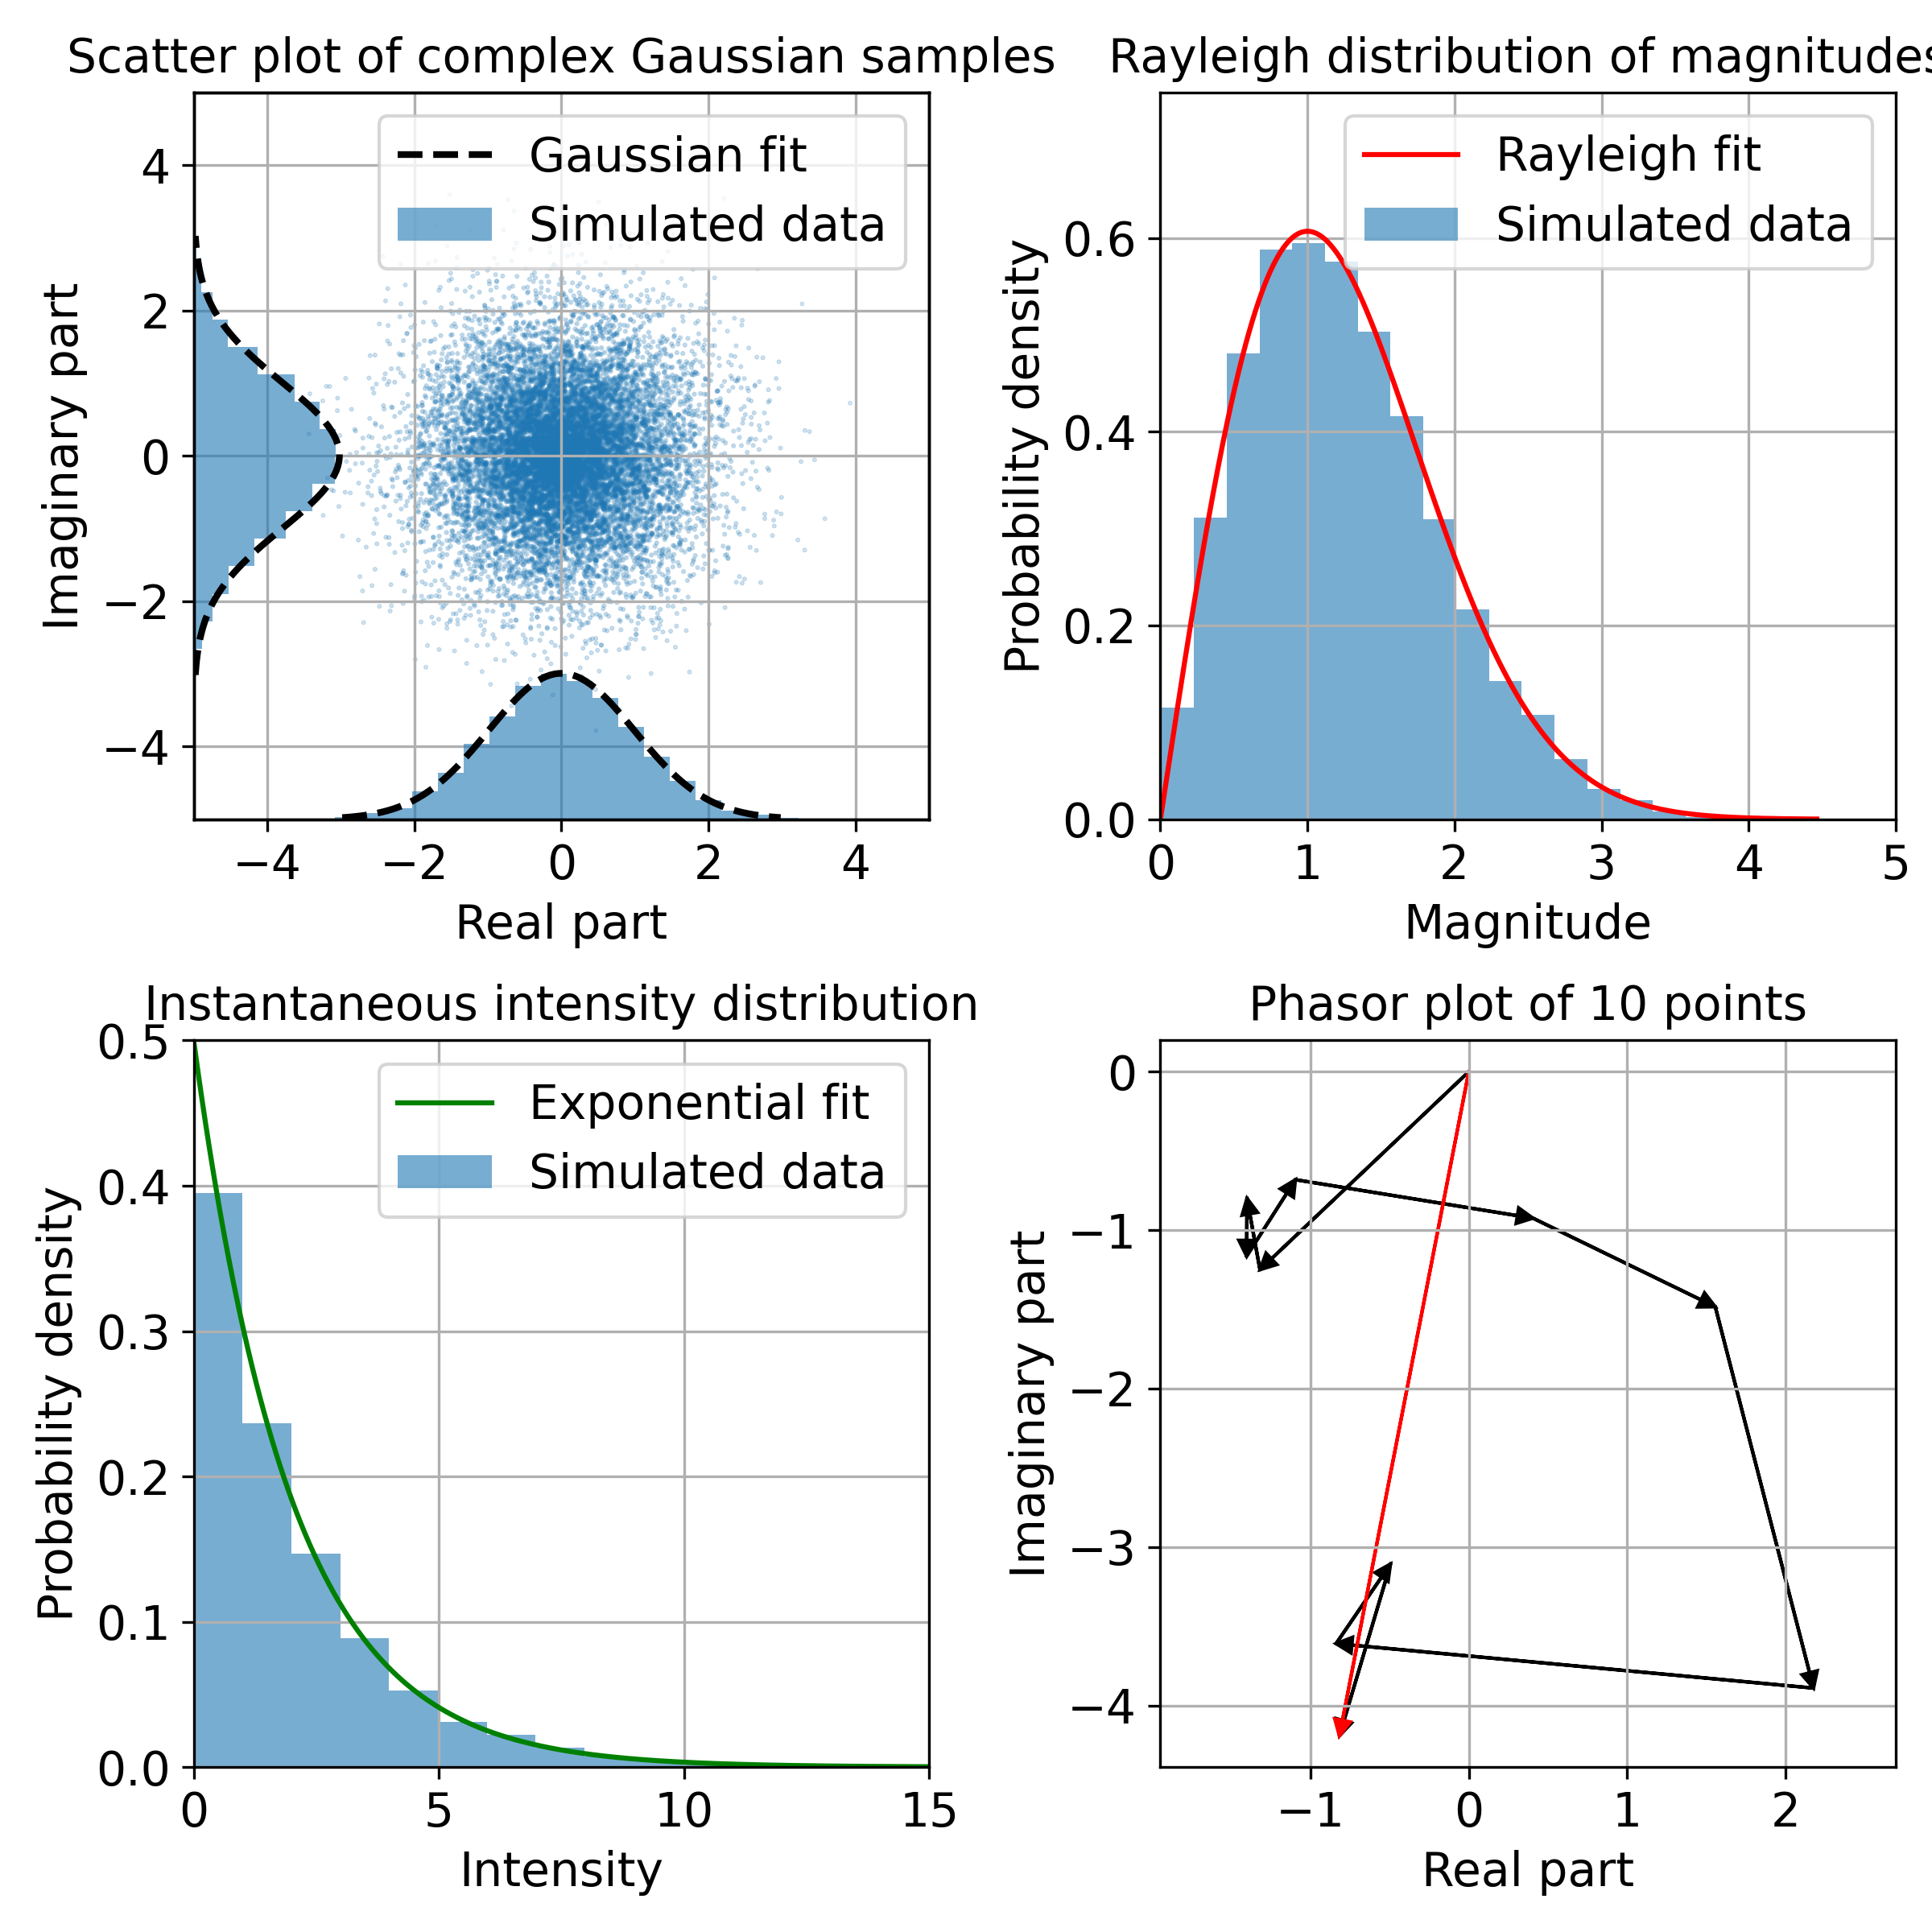
\includegraphics[width=0.75\linewidth]{content/images/Statistical_Optics/gaussian_process.png}
        \captionsetup{justification=centering}
        \caption{Gaussian random process visualisation, dispersion equals unity. Upper left subplot is 10000 samples marked at imaginary plane, upper right subplot Rayleigh distribution, lower left subplot negative exponent distribution, lower right subplot random phasor plotted from ten point.}
        \label{Fig:gaussian_process}
    \end{figure}
    This distribution is called the \textit{Rayleigh probability distribution}. In the last equation, the dependence on $\phi$ is not presented explicitly, which implies that the phase is distributed uniformly for all values ($0 \leq \phi \leq 2 \pi$), i.e.:
    \begin{align}
        p(\phi) = \cfrac{1}{\sqrt{2 \pi}}.
    \end{align}
    One can also consider probability density function for the \textit{instantaneous intensity}:
    \begin{align}
        I(t) = A^2(t)
    \end{align}
    and using the law for probability functions transformations I obtain:
    \begin{align}
        p(I) = \frac{1}{\langle I \rangle} e^{-I/\langle I \rangle},
    \end{align}
    where $\langle I \rangle = 2 \sigma$. This is distribution is negative exponential distribution. \rr{…and…need to have a conclusion}

    \rr{…it sounds ragged…}
    Gaussian random processes play a fundamental role in synchrotron radiation (SR) and self-amplified spontaneous emission free-electron laser (SASE FEL) radiation, and more generally, in statistical optics. From this point forward, I will assume that the processes dealt with in this thesis possess Gaussian statistics, with several exceptions discussed separately. Now, I will focus on extending the definition of stationarity to a broader class to account for the time-confined nature of SR and SASE FEL radiation.
    
\subsection{Quasi-stationary approximation}

    Although many day-to-day sources of radiation can be categorized as stationary or ergodic, non-stationary processes play a pivotal role in science. However, developing a generalized theory for non-stationary processes and deriving practical laws is very challenging. Nevertheless, there is a class of sources that can be described in the same manner similar to stationary ones. This kind of source are referred to as quasi-stationary. At this point, I will slightly deviate from the usual presentation of statistical optics concepts, like in~\cite{mandel_optical_1995, goodman_statistical_2015}, and delve into the concept of quasi-stationary. As the name suggests, quasi-stationary processes share the most of statistical properties with stationary ones, but they start and finish at specific points in time. Quasi-stationary processes appear to be stationary only within a certain interval of time, which is much smaller than their overall duration.
    
    So, if one observes radiation intensity at some point in space and record it over time then the ensemble average will be:
    \begin{align}
        I(t) \coloneqq \langle I(t) \rangle = \lim_{N\to\infty} \frac{1}{N}\sum_{i=1}^{N} E^{[i]}(t)E^{*[i]}(t)
    \end{align}
    $I(t)$ is the time envelope of the radiation and depends on time. Then I write the auto-correlation function:
    \begin{align}
        \Gamma(t_1, t_2) = \langle E(t_1)E^*(t_2) \rangle = \lim_{N\to\infty} \frac{1}{N}\sum_{i=1}^{N} E^{[i]}(t_1)E^{*[i]}(t_2)
    \end{align}
    At this point, I have not defined anything except for the fact that $I(t) \neq C$ and does depend on time, where $C$ is some constant. Then, introducing the normalized version of the auto-correlation function $\Gamma(t_1, t_2)$:
    \begin{align}
        g(t_1, t_2) = \frac{\langle E(t_1)E^*(t_2)\rangle}{\sqrt{\langle |E(t_1)|^2\rangle \langle |E^*(t_2)|^2\rangle}} = \frac{\Gamma(t_1, t_2)}{\sqrt{ I(t_1) I(t_2)}}.
    \end{align} 
    and rewriting this as: 
    \begin{align}
        \Gamma(t_1, t_2) = g(t_1, t_2) \sqrt{I(t_1) I(t_2)}.
    \end{align}
    I notice that for a quite large span of the process $g(t_2, t_1)$ only depends on the time difference $\Delta t = t_2 - t_1$. Having this, I obtain:
    \begin{align}
        \Gamma(t_1, t_2) = g(t_2 - t_1) \sqrt{I(t_1) I(t_2)}.
        \label{Eq:Strict_quasi_stationarity}
    \end{align}
    The radiation sources that have this kind of auto-correlation function I will call quasi-stationary, but there is a "weaker" definition of quasi-homogeneity. If one assumes that the width $g(t_2 - t_1)$ is much smaller than the scale of $I(t)$, then the result is an even simpler expression:
    \begin{align}
        \Gamma(t_1, t_2) = g(t_2 - t_1)I\bigg(\frac{t_1 + t_2}{2}\bigg)
        \label{Eq:weak_quasi_stationarity}
    \end{align}
    This representation of radiation sources is to some extent similar to quasi-homogeneity in the transverse domain~\cite{goodman_statistical_2015}. To my best knowledge, there are only a few mentions of Eq.~\ref{Eq:weak_quasi_stationarity}~\cite{lajunen_quasi-stationary_2006, ahad_quasi-monochromatic_2017} in optics community and authors of~\cite{geloni_statistical_2006} resulted in this expression for synchrotron radiation. Up to this point, I have not related these definition to real-world physical examples. First, I aim to derive another very useful properties of such processes and then provide an example, specifically, synchrotron radiation, which in most practical cases follows these definitions.

    \rr{…need to extend the content of this section a little bit}
    
\subsection{Cross-spectral density and generalized Wiener-Khinchin theorem}
    
    Continuing derivations, now I look at the correlation function in frequency domain. By definition I auto-correlate the Fourier images $\bar{E}(\omega)$ of the fields $E(t)$ at different frequencies $\omega_1$ and $\omega_2$:
    \begin{align}
        \langle \bar{E}(\omega_1)\bar{E}^*(\omega_2) \rangle = \frac{1}{(2 \pi)^2} \iint \limits_{-\infty}^{\infty} \langle E(t_1)E^*(t_2) \rangle e^{i \omega_1 t_1 - \omega_2 t_2} dt_1 dt_2, 
        \label{Eq:cross_spectral_density_dif}
    \end{align}
    where I brought the ensemble averaging under the integral sign. Then by using the expression Eq.~\ref{Eq:weak_quasi_stationarity} and substituting this in Eq.~\ref{Eq:cross_spectral_density_dif} I obtain:
    \begin{align}
        \langle \bar{E}(\omega_1)\bar{E}^*(\omega_2) \rangle = \frac{1}{(2 \pi)^2} \iint \limits_{-\infty}^{\infty}  g(t_2 - t_1)I\bigg(\frac{t_1 + t_2}{2}\bigg) e^{i \omega_1 t_1 - \omega_2 t_2} dt_1 dt_2.
    \end{align}
    I this point it makes sense to exchange variables $t_1, t_2$ for $\Delta t = t_2 - t_1$ and $\bar{t} = (t_2 + t_1)/2$. Now it is evident that it is possible to factorize the integral:
    \begin{align}
        \langle \bar{E}(\omega_1)\bar{E}^*(\omega_2) \rangle = \frac{1}{(2 \pi)^2} \int \limits_{-\infty}^{\infty}  g(\Delta t) e^{i \bar{\omega} \Delta t} d \Delta t  \int \limits_{-\infty}^{\infty} I(\bar{t}) e^{-i \Delta \omega \bar{t}} d\bar{t} = \bar{I}(\bar{\omega})f_{\omega}(\Delta \omega).
        \label{Eq:general_WKh_t}
    \end{align}
    This result in Eq.~\ref{Eq:general_WKh_t} I will refer to as the generalized Wiener-Khinchin theorem, although it is difficult to find this result elsewhere except for~\cite{geloni_statistical_2006} \rr{really? check again} in application to synchrotron radiation. A similar expression can be formulated for stationary radiation where $I(\bar{t})$ is constant $C$ and one obtains the integral:
    \begin{align}
        \langle \bar{E}(\omega_1)\bar{E}^*(\omega_2) \rangle = \frac{C}{(2 \pi)^2} \int \limits_{-\infty}^{\infty}  g(\Delta t) e^{i \bar{\omega} \Delta t} d \Delta t  \int \limits_{-\infty}^{\infty} e^{-i \Delta \omega \bar{t}} d\bar{t} = \bar{I}(\bar{\omega})\delta(\Delta \omega),
        \label{Eq:WKh_t_derivation}
    \end{align}
    where the latter integral equals the Dirac delta function: $\delta(\Delta \omega)$, and one can recognize that the radiation spectral density or just spectrum is related to the auto-correlation function via a Fourier transform.
    \begin{align}
        \bar{I}(\bar{\omega}) = \frac{1}{(2 \pi)^2} \int \limits_{-\infty}^{\infty}  g(\Delta t) e^{i \bar{\omega} \Delta t} d \Delta t,
        \label{Eq:WKh_t}
    \end{align}
    Both expression under Eqs.~\ref{Eq:general_WKh_t} and~\ref{Eq:WKh_t} play an essential role in coherence theory on an equal footing with the van Cittert-Zernike theorem, which I present in the next sections.

\section{Transverse coherence properties of quasi-stationary sources}
\label{Sec:Transverse coherence properties of quasi-stationary sources}
    
    Previously, I only considered sources in the time-frequency domain, while real fields exist in three-dimensional space. In this section, I will introduce transverse variables into the autocorrelation function. Then, I will classify the types of sources in terms of the factorizability of the cross-spectral density function, in a manner very similar to what I have done for the longitudinal domain. After this, I will provide proof of the van Cittert-Zernike theorem and its generalized version for quasi-homogeneous sources. This chapter will be the last one on the general laws of statistical optics, and it will be followed by practical applications of the theory to synchrotron and free-electron laser.

\subsection{Adding transverse domain}

    In the previous section, the signal was effectively observed through a pinhole. As I consider optical phenomena, not many of them truly occur only in the time-frequency domain -- the signal's propagation direction -- and extend into the transverse domains as well. Therefore, the expressions I previously provided should be adjusted accordingly to correctly reflect the statistical properties in transverse dimensions.
    Looking at Eq.~\ref{Eq:general_WKh_t},  I assume that $I(\bar{t})$ does not depend on transverse coordinates and I re-denote this distribution to $f(\bar{t})$. All the dependence on transverse variables $\vec{r}_1, \vec{r}_2$ goes to the $g_t$.
    \begin{align}
        \Gamma_{\omega}(\vec{r}_1, \vec{r}_2, \omega_1, \omega_2) = \frac{1}{(2 \pi)^2} \int \limits_{-\infty}^{\infty}  g_t(\vec{r}_1, \vec{r}_2, \Delta t) e^{i \bar{\omega} \Delta t} d \Delta t  \int \limits_{-\infty}^{\infty} f(\bar{t}) e^{-i \Delta \omega \bar{t}} d\bar{t} = G_{\omega}(\vec{r}_1, \vec{r}_2, \bar{\omega})\bar{f}(\Delta \omega),
        \label{Eq:}
    \end{align}    
    This representation results in the appearance of the cross-spectral density function $G_{\omega}(\vec{r}_1, \vec{r}_2, \bar{\omega})$ in a manner similar to that done for stationary sources but along with $\bar{f}(\Delta \omega)$ function that describes spectral correlation.

\subsection{Cross-spectral function distribution at the source}

    Continuing the reasoning on the transverse domain of the radiation, the normalized version of the cross-spectral density function has the following form:
    \begin{align}
        g(\vec{r}_1, \vec{r}_2, \omega; 0) = \frac{G(\vec{r}_1, \vec{r}_2, \omega; 0)}{\sqrt{I(\vec{r}_1, \omega; 0)I(\vec{r}_2, \omega; 0)}}.
    \end{align}
    Then, one can express cross-spectral density function as the following:
    \begin{align}
        G(\vec{r}_1, \vec{r}_2, \omega; 0) =  g(\Delta \vec{r}, \omega; 0){\sqrt{I(\vec{r}_1, \omega)I(\vec{r}_2, \omega; 0)}},
        \label{Eq:quasi_homogeneous_source_strong}
    \end{align}
    here I assumed that coherence length is distributed homogeneously across the intensity distribution in a similar way to what I have done in Eq.~\ref{Eq:Strict_quasi_stationarity}. This means that the width of $g(\Delta \vec{r}, \omega; 0)$ does not change across the intensity distribution. This kind of radiation source is called quasi-homogeneous according to another classical textbook~\cite{goodman_statistical_2015}. I can simplify the expression further and make further assumptions on the width of the $g(\Delta \vec{r}, \omega; 0)$ function to be much smaller than the radiation envelope $I(\bar{\vec{r}}, \omega; 0)$, again exactly similarly as was done for the longitudinal domain:
    \begin{align}
        G(\vec{r}_1, \vec{r}_2, \omega; 0) =  g(\Delta \vec{r}, \omega; 0)I(\vec{\bar{r}}, \omega).
        \label{Eq:quasi_homogeneous_source_weak}
    \end{align}
    In the limit case of fully incoherent source this degenerate to the following expression:
    \begin{align}
        G(\vec{r}_1, \vec{r}_2, \omega; 0) =  I(\vec{\bar{r}}, \omega; 0)\delta(\Delta \vec{r}),
        \label{Eq:incoherent_source}        
    \end{align}
    where the Dirac delta function is introduced. This kind of source describes fully incoherent sources or sources where the resolution of the optical system is larger than $g(\Delta \vec{r})$,~\cite{goodman_statistical_2015}.
    
\subsection{Propagation law for cross-spectral density function in free space}

    Another essential problem in coherence theory concerns the propagation of coherence properties through an optical system, which includes various optical elements interspaced with free space. By its nature, a single statistical realization of a field from a random process behaves identically to any other field and can be propagated in the same way, adhering to the wave equation. Looking ahead to the narrative of this thesis, one effective method to calculate the field and its statistical properties upon propagation is to directly apply the corresponding propagator—or a sequence of propagators—through the optical system. Although this approach is practical, it can also be somewhat cumbersome. It necessitates propagating each field sample separately or deriving an analytical expression for the corresponding propagator. Nevertheless, this method is used in many numerical codes for radiation propagation, including Synchrotron Radiation Workshop (SRW)~\cite{chubar_accurate_1998}.
 
    In the simplified scenario of just free space, it is possible to derive a highly useful law describing how the cross-spectral density function or the mutual coherence function evolves. This case is particularly applicable for estimating coherence properties at the entrance of the optical system. Typically, there is free space between the radiation source and the entrance of an optical system. I begin by examining the wave equation in free space:
    \begin{align}
        \nabla^2_1 \vec{E}(\vec{r}_1, t_1) - \cfrac{1}{c^2} \frac{\partial^2 \vec{E}(\vec{r}_1, t_1)}{\partial t_1^2} = 0
        \label{Eq:wave_eq}
    \end{align}
    By multiplying this with $\vec{E}^(\vec{r}_2, t_2)$, where $^*$ denotes the complex conjugate, and then incorporating it under the differentiation signs:
    \begin{align}
        \nabla^2_1 \big[\vec{E}(\vec{r}_1, t_1) \vec{E}(\vec{r}_2, t_2)\big]- \cfrac{1}{c^2} \frac{\partial^2 \big[\vec{E}(\vec{r}_1, t_1) \vec{E}(\vec{r}_2, t_2)\big]}{\partial t_1^2} = 0.
    \end{align}
    and then by ensemble averaging this equation, and noting that the averaging operation can be interchanged with differentiation, I obtain:
    \begin{align}
        \nabla^2_1 \Gamma(\vec{r}_1, \vec{r}_2, t_1, t_2)  - \cfrac{1}{c^2} \frac{\partial^2 \Gamma(\vec{r}_1, \vec{r}_2, t_1, t_2)}{\partial t_1^2} = 0,
    \end{align}
    To close this differential system, one can derive the complementary equation in the same manner:
    \begin{align}
        \nabla^2_2 \Gamma(\vec{r}_1, \vec{r}_2, t_1, t_2)  - \cfrac{1}{c^2} \frac{\partial^2 \Gamma(\vec{r}_1, \vec{r}_2, t_1, t_2)}{\partial t_2^2} = 0,
    \end{align}
    By taking the Fourier transform of both sides, I obtain a system for the cross-spectral density function $G(\vec{r}_1, \vec{r}_2, \omega)$ that is:
    \begin{align}
        \nabla^2_1 G(\vec{r}_1, \vec{r}_2, \omega) + k^2 G(\vec{r}_1, \vec{r}_2, \omega) = 0\\
        \nabla^2_2 G(\vec{r}_1, \vec{r}_2, \omega) + k^2 G(\vec{r}_1, \vec{r}_2, \omega) =0 .
    \end{align}
    where I divided each equation by $\bar{f}(\Delta \omega)$. This system of two Helmholtz equations has a known solution. Assuming that we know the distribution $G(\vec{r}'_1, \vec{r}'_2, \omega)$ in the $S$ plane, where $z=0$, we can solve this system using the Green's function for the Helmholtz equation with Dirichlet boundary conditions. This approach allows us to derive the following law for propagating the cross-spectral density function~\cite{mandel_optical_1995}:
    \begin{align}
        G(\vec{r}_1, \vec{r}_2, \omega) = \bigg(\cfrac{k}{ 2 \pi} \bigg)^2 \iint_{z=0} G(\vec{r}'_1, \vec{r}'_2, \omega) \cfrac{e^{i k (R_2 - R_1)}}{R_1 R_2} \cos(\theta_1) \cos(\theta_2) d^2r'_1 d^2r'_2
        \label{Eq:G_propagation_law}
    \end{align}
    \begin{wrapfigure}{r}{0.5\textwidth}
        \centering
        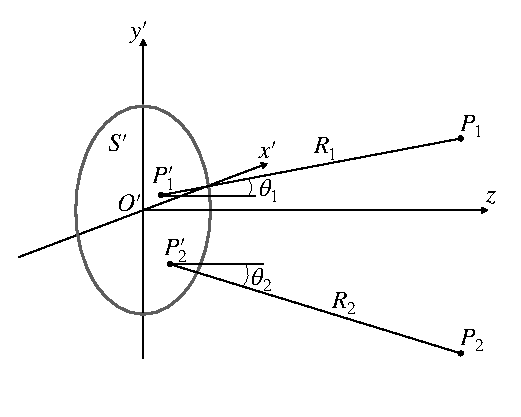
\includegraphics[width=0.95\linewidth]{content/images/Statistical_Optics/coh_prop_scheme.pdf}
        \captionsetup{justification=centering}
        \caption{Geometry of the cross-spectral density propagation in the free-space. Adapted from~\rr{cite}}
        \label{Fig:coh_prop_scheme}
    \end{wrapfigure}
    This expression is foundational for deriving the van Cittert-Zernike theorem, which I will discuss in the next section. Historically, the van Cittert-Zernike theorem was formulated using Huygens' principle, resulting in an expression for the mutual intensity function~\cite{van_cittert_wahrscheinliche_1934, zernike_concept_1938}. Interestingly, it should be noted that the cross-spectral density obeys the same laws as the mutual intensity function $J(\vec{r}_1, \vec{r}_2) = g_t(\vec{r}_1, \vec{r}_2, \Delta t = 0)$~\cite{goodman_statistical_2015, mandel_optical_1995}. It is important to remember that this holds true only for quasi-monochromatic sources. Therefore, I will continue to present the results for the theorem using the cross-spectral density.

\subsubsection{The van Cittert-Zernike theorem}
    Equation~\ref{Eq:G_propagation_law} is highly general and can be applied to any propagating field to calculate its cross-spectral distribution upon propagation. However, this integral can be further simplified to derive practical formulas for specific types of sources—namely, fully incoherent and partially coherent sources under the quasi-homogeneous approximation that I have introduced in Eqs.~\ref{Eq:quasi_homogeneous_source_weak},~\ref{Eq:incoherent_source}. 
    
    Assuming the paraxial approximation, I can write the following expression for the mutual intensity function derived from Eq.~\ref{Eq:G_propagation_law}:
    \begin{align}
        G(\vec{r}_1, \vec{r}_2, \omega) = \bigg(\cfrac{k}{ 2 \pi} \bigg)^2 \iint_{\mathcal{S}} G(\vec{r}'_1, \vec{r}'_2, \omega) \cfrac{e^{i k (R_2 - R_1)}}{R_1 R_2}d^2r'_1 d^2r'_2
        \label{Eq:G_propagation_law_4_VCZ}
    \end{align}
    \begin{figure}[h!]
        \centering
        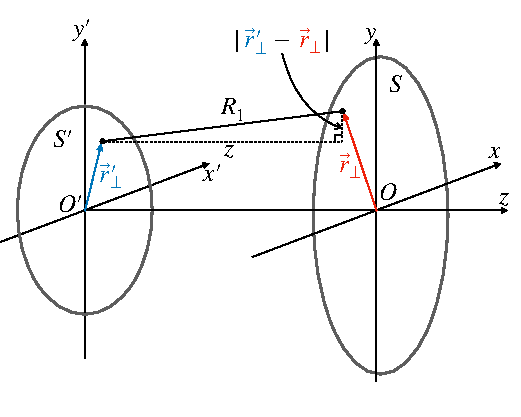
\includegraphics[width=0.5\linewidth]{content/images/Statistical_Optics/coh_prop_scheme_2.pdf}
        \captionsetup{justification=centering}
        \caption{Geometry of the cross-spectral density propagation in the free-space. Adapted from~\rr{cite}.}
        \label{Fig:coh_prop_scheme_2}
    \end{figure}
    If the cross-spectral density function is observed in the far zone Eq.~\ref{Eq:G_propagation_law_4_VCZ} can be further simplified using the relations:
    \begin{align}
        \begin{array}{c}
            R_{1, 2}\approx  z + \cfrac{|\vec{r}'_{1, 2{\perp}} - \vec{r}_{1, 2{\perp}}|^2}{2z}\\
            \\
            R_{1}R_{1} \approx z^2
        \end{array}
        \label{Eq:R1R2_simp}
    \end{align}
    for simplicity of the notation it make sense to redefine $\vec{r}_{1, 2} :=\vec{r}_{1, 2{\perp}}$ and the same for $\vec{r}'_{1, 2} :=\vec{r}'_{1, 2{\perp}}$ (but only till the end of the current Section).

    Now I would like to simplify $R_2 - R_1$ in the exponent. Using first relation in Eq.~\ref{Eq:R1R2_simp}:
    \begin{align}
        R_2 - R_1 = \cfrac{1}{2z} \bigg(|\vec{r}_{2}|^2 - 2|\vec{r}_{2} \cdot \vec{r}'_{2}| + |\vec{r}'_{2}|^2 - |\vec{r}_{1}|^2 + 2|\vec{r}_{1} \cdot \vec{r}'_{1}| - |\vec{r}'_{1}|^2\bigg)
    \end{align} 
    and introducing new variables $\vec{\bar{r}} = \vec{r}_1 - \vec{r}_2$ and $\Delta\vec{r} = (\vec{r}_2 + \vec{r}_1)/2$ and the same for the primed set of variables, this leads me to: 
    \begin{align}
        \begin{array}{c}
        |\vec{r}_{2}|^2 - |\vec{r}_{1}|^2 = -2\vec{\bar{r}}\cdot\Delta\vec{r} \\
        |\vec{r}'_{2}|^2 - |\vec{r}'_{1}|^2 = -2\vec{\bar{r}}'\cdot\Delta\vec{r}' \\
        |\vec{r}_{1} \cdot \vec{r}'_{1}| - |\vec{r}_{2} \cdot \vec{r}'_{2}| = \vec{\bar{r}}\cdot\Delta\vec{r}' + \vec{\bar{r}}'\cdot\Delta\vec{r},
        \end{array}
    \end{align}
    where $\_ \cdot \_$ denotes the scalar product. Then I substitute this in Eq.~\ref{Eq:G_propagation_law_4_VCZ} and obtain:
    \begin{align}
        G(\vec{\bar{r}}, \Delta\vec{r}, \omega; 0) = \bigg(\cfrac{k}{ 2 \pi} \bigg)^2 \cfrac{e^{-\frac{i k}{z} \vec{\bar{r}}\cdot\Delta\vec{r}}}{z^2}     \iint_{\mathcal{S}} G(\vec{\bar{r}}', \Delta\vec{r}', \omega, z) e^{\frac{i k}{z} (\vec{\bar{r}}\cdot\Delta\vec{r}' + \Delta\vec{r}\cdot\vec{\bar{r}}')} d\vec{\bar{r}}' d\Delta\vec{r}' 
        \label{Eq:VCZ_general_form}
    \end{align}
    Here, I neglected the term $2\vec{\bar{r}}'\cdot\Delta\vec{r}'$ in the exponent under assumption condition $\vec{\bar{r}}'\cdot\Delta\vec{r}'/ (\lambda z) \ll 1$, which basically can be interpreted as placing the observation plane ($S'$) in far zone.
    
    Using this definition of fully incoherent source and substituting this in Eq.~\ref{Eq:VCZ_general_form} I obtains:
    \begin{align}
        G(\vec{\bar{r}}, \Delta\vec{r}, \omega; z) &= \cfrac{e^{- i \frac{k}{z} \vec{\bar{r}}\cdot\Delta\vec{r}}}{(\lambda z)^2} \iint_{\mathcal{S}} I(\vec{\bar{r}}', \omega)\delta(\Delta \vec{r}') e^{i \frac{k}{z} (\vec{\bar{r}}\cdot\Delta\vec{r}' + \vec{\bar{r}}'\cdot\Delta\vec{r})} d\vec{\bar{r}}' d\Delta\vec{r}' \nonumber = \\
        &\fcolorbox{black}{yellow!30}{\rule[-4ex]{0pt}{10ex}$\displaystyle \stackrel{\text{van Cittert-Zernike theorem}}{\cfrac{e^{-i \frac{k}{z} \vec{\bar{r}}\cdot\Delta\vec{r}}}{(\lambda z)^2} \int_{\mathcal{S}} I(\vec{\bar{r}}', \omega) e^{i \frac{k}{z} \vec{\bar{r}}'\cdot\Delta\vec{r}} d\vec{\bar{r}}'}$}
        \label{Eq:VCZ_incoherent}
    \end{align}
    This is the original result of the van Cittert-Zernike theorem but the theorem can be extended for a more general source representation under Eq.~\ref{Eq:quasi_homogeneous_source_weak}. Again using integral in Eq.~\ref{Eq:VCZ_general_form} and substituting in it the expression from Eq.~\ref{Eq:quasi_homogeneous_source_weak} I obtain:
    \begin{align}
        G(\vec{\bar{r}}, \Delta\vec{r}, \omega; z) &=  \cfrac{e^{-i \frac{k}{z} \vec{\bar{r}}\cdot\Delta\vec{r}}}{(\lambda z)^2} \iint_{\mathcal{S}} g(\Delta \vec{r}', \omega; 0)I(\vec{\bar{r}}', \omega) e^{i \frac{k}{z} (\vec{\bar{r}}\cdot\Delta\vec{r}' + \vec{\bar{r}}'\cdot\Delta\vec{r})} \, d\vec{\bar{r}}' \, d\Delta\vec{r}' \nonumber =\\
        &\fcolorbox{black}{yellow!30}{\rule[-4ex]{0pt}{10ex}$\displaystyle \stackrel{\text{generalised van Cittert-Zernike theorem}}{\cfrac{e^{-i \frac{k}{z} \vec{\bar{r}}\cdot\Delta\vec{r}}}{(\lambda z)^2} \int_{\mathcal{S}} g(\Delta \vec{r}', \omega; 0) e^{-i \frac{k}{z} \vec{\bar{r}}\cdot\Delta\vec{r}'} \, d\Delta\vec{r}'  \int_{\mathcal{S}} I(\vec{\bar{r}}', \omega) e^{i \frac{k}{z} \vec{\bar{r}}'\cdot\Delta\vec{r}} \, d\vec{\bar{r}}'}$}
        \label{Eq:VCZ_partially_coherent}
    \end{align}
    \begin{figure*}[h!]
      \centering
      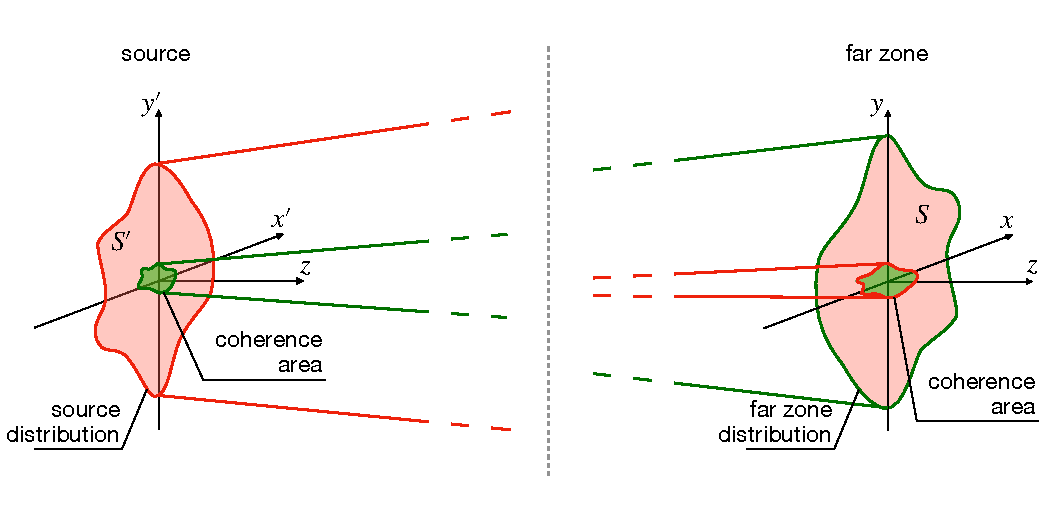
\includegraphics[width=0.95\linewidth]{content/images/Statistical_Optics/VCZ_scheme.pdf}
      \captionsetup{justification=centering}
      \caption{Visual representation of the generalised van Cittert-Zernike theorem. }
      \label{Fig:coh_prop_scheme}
    \end{figure*}
    \begin{figure}[h!]
        \centering
        \begin{tikzpicture}[
            % Define styles
            node distance=2cm,
            mynode/.style={
              shape=ellipse,
              draw,
              text width=2.5cm,
              align=center
            },
            bluearrow/.style={
              <->,
              >=latex,
              blue,
              thick
            },
            redarrow/.style={
              <->,
              >=latex,
              red,
              thick
            },
            bluetext/.style={
              text=blue
            },
            redtext/.style={
              text=red
            }
          ]
        
          % Nodes
          \node[mynode] (g0) {$g(\Delta\mathbf{\hat{r}}; \mathbf{0})$};
          \node[mynode, right=of g0] (I0) {$I(\mathbf{\hat{r}}; \mathbf{0})$};
          \node[mynode, below=of g0] (gz) {$\dfrac{g( \Delta\mathbf{\hat{\theta}}; \mathbf{\hat{z}})}{\exp[i\mathbf{\hat{z}} \Delta\mathbf{\hat{\theta}} \cdot \mathbf{\theta}]}$};
          \node[mynode, right=of gz] (Iz) {$I(\mathbf{\hat{\theta}}; \mathbf{\hat{z}})$};
        
          % Arrows with FT labels
          \draw[bluearrow] (g0) -- (Iz) node[pos=0.25, above, bluetext] {FT};
          \draw[redarrow] (gz) -- (I0) node[pos=0.75, above, redtext] {FT};
        \end{tikzpicture}
        \caption{Relations between intensity and cross-spectral distributions at the source and in the far zone that van Cittert-Zernike theorem and its inverse version set.}
        \label{Fig:VCZ_scheme}
    \end{figure}
    This is a result for a partially coherent source with cross-spectral density distribution as given in Eq.~\ref{Eq:quasi_homogeneous_source_weak}. Surely, it is easy to show that the inverse version of the van Cittert-Zernike theorem holds as well. So, I present all the relations in the diagram in Fig.~\ref{Fig:VCZ_scheme}. The van Cittert-Zernike theorem (and its generalized version) provides a very practical relation between the source size and the observed coherence spot in the far zone and forms the basis for coherence theory for studying synchrotron radiation sources.

    \rr{discuss more on the results}

\section{Coherence properties of synchrotron radiation}

    In this section, I will explore the general theory of synchrotron radiation coherence, following the framework presented in~\cite{geloni_statistical_2006}. This framework results in practical expressions for calculating the correlation function that are well-suited for numerical implementation. This numerical implementation resembles Monte-Carlo-like methods, where the contribution from each particle is calculated separately and then summed up. This is discussed in detail in the corresponding sections of Paper II.

    Based on the theory developed in this section, I will provide the theoretical reasoning and introduce algorithms for calculating radiation using Gaussian field generators based on white noise \rr{again, Gaussian noise, white noise? should be one term across the thesis} later in the chapter. First, I present an algorithm for fully incoherent radiation and demonstrate its application in Paper I, focusing on the image formation properties of a pinhole camera at a synchrotron facility. Then, I extend it to the case of partially coherent radiation and present the results in Paper II, followed by Paper III, where I consider an algorithm for generating radiation with arbitrary phase space distribution. Each development stage of the algorithm will be preceded by a dedicated "heuristic" section, outlining the idea behind the algorithm.

    The classical textbook on statistical optics~\cite{mandel_optical_1995} provides a wave equation for radiation from a fluctuating scalar source in the following form:
    \begin{align}
        c^2 \nabla^2 \vec{E}(\vec{r}, t) - \frac{\partial^2 \vec{E}(\vec{r}, t)}{\partial t^2} = -4 \pi c^2 Q(\vec{r}, t).
        \label{Eq:mandel_Eq}
    \end{align}
    It then provides an expression for propagating the radiation from the source based on the propagation law of the correlation function. This means that the correlation function at some position along the optical axis can be expressed as an integral using the correlation function of the source:
    \begin{align}
        \Gamma_Q(\vec{r}_1, \vec{r}_2, t_1, t_2) = \langle  Q(\vec{r}_1, t_1)  Q^*(\vec{r}_2, t_2) \rangle.
        \label{Eq:wave_eq_Mandel}
    \end{align}
    \rr{STOPPED HERE}
    This calculation is complicated by the fact that the nature of $Q(\vec{r}, t)$ remains obscured. For example, to describe a thermal source, radiation must be calculated using quantum mechanics, making it unclear how to properly present the wave equation in Eq.~\ref{Eq:wave_eq_Mandel}. Fortunately, synchrotron radiation from a relativistic electron beam is governed solely by classical electrodynamics, allowing for writing an explicit equation in the same manner as Eq.~\rr{}, but accounting for the whole electron beam:
    \begin{align}
        c^2 \nabla^2 \vec{E} - \frac{\partial^2 \vec{E}}{\partial t^2} = - 4 \pi c^2 \vec{\nabla} (-e) \sum_{i=1}^{N_e}\delta(\vec{r} - \vec{r}_i'(t)) + 4 \pi (-e) \sum_{i=1}^{N_e}\frac{\partial (\vec{v}_i(t)\delta(\vec{r} - \vec{r}_i'(t)))}{\partial t}.
    \end{align}
    This equation represents a stochastic partial differential equation where the right-hand side depends on random variables, such as the coordinates and velocities of electrons within the electron beam's phase space. Solving this equation in the context of stochastic partial differential equations demands substantial analytical effort, if not impossible at the current moment.

    This problem can be simplified by employing the superposition principle of electrodynamics. As demonstrated in Chapter~\ref{Chapter:Undulator radiation imaginary source peculiarities}, one can easily solve the equation for a single electron. One can obtain the final solution for the field by summing up the contributions from all electrons. In numerical simulations, this approach requires solving $N_e \times N_b$ equations for single electrons, where $N_e$ is the number of electrons and $N_b$ is the number of statistical realizations. Nevertheless, analytically, this approach can lead to very useful and practical equations for the coherence properties of synchrotron radiation, which I will discuss in the next section.
    
\subsection{Cross-spectral density functions for synchrotron radiation}   
    
    This section mainly follows the reasoning given in~\cite{geloni_statistical_2006}. As it has been discussed, the field from the whole electron beam can be written as the sum of the field of individual electrons:
    \begin{align}
        E_b(z, \vec{r}, t) = \sum_{k=1}^{N_e} E(\vec{\eta}_k, \vec{l}_k, z, \vec{r}, t - t_k), 
    \end{align}
    where $\vec{\eta}_k$ is an electron deflection, $\vec{l}_k$ its offset and $t_k$ -- arrival time with respect to some reference time. It is more practical to consider this field in frequency domain that will be rewritten as the following: 
    \begin{align}
        \bar{E}_b(z, \vec{r}, \omega) = \sum_{k=1}^{N_e} \bar{E}(\vec{\eta}_k, \vec{l}_k, z, \vec{r}, \omega)e^{i \omega t_k}.
        \label{Eq:ebeam_rad_omega}
    \end{align}   
    Here I note that all $\bar{E}$ have the same distribution for all $k$ and have finite mean and dispersion. Additionally, the arrival times of the electrons $t_k$ are statistically independent of each other and do not depend on $\vec{\eta}_k, \vec{l}_k$.
    
    I assume that the length of the electron beam $\sigma_T c$ is much larger than the wavelength: \rr{$\omega \sigma_T \ll 1$ ??}. This leads to the approximation that the phase is distributed uniformly in the interval $(0, 2\pi)$. The case $\omega \sigma_T \gg 1$ refers to an effect called coherent synchrotron radiation (CSR), which I do not consider in this thesis.
    
    With these assumptions, I can prove that the field $\bar{E}_b(z, \vec{r}, \omega)$ actually follows complex Gaussian random process statistics, or simply saying throughout this thesis Gaussian statistics. Indeed, with the help of the central limit theorem, it is clear that the sum of the random functions in Eq.~\ref{Eq:ebeam_rad_omega} will result in the real and imaginary parts of $\bar{E}_b$ following Gaussian statistics.
    
    Writing the cross-spectral density function of the first order of the field $\bar{E}_b$:
    \begin{align}
        \Gamma_\omega (z, \vec{r}_1, \vec{r}_2, \omega_1, \omega_2) = \langle \bar{E}_b(z, \vec{r}_1, \omega_1) \bar{E}^*_b(z, \vec{r}_1, \omega_1) \rangle,
        \label{Eq:Gamma_omega}
    \end{align} 
    and substituting Eq.~\ref{Eq:ebeam_rad_omega} in Eq.~\ref{Eq:Gamma_omega} I obtain:
    \begin{align}
        \Gamma_\omega (z, \vec{r}_1, \vec{r}_2, \omega_1, \omega_2) = \bigg\langle 
        \sum_{m,n=1}^{N_e} \bar{E}(\vec{\eta}_m, \vec{l}_m, z, \vec{r}, \omega_1)\bar{E}^*(\vec{\eta}_n, \vec{l}_n, z, \vec{r}, \omega_2)e^{i (\omega_1 t_m - \omega_2 t_n)}
        \bigg\rangle
    \end{align}
    At this point, it is worth noting that higher-order correlation functions of a Gaussian random process can be expressed with the help of the moment theorem, as mentioned in Section~\ref{Sec:Gaussian random processes}. This is a fundamental property of Gaussian random processes and a central one for this thesis.
    
    Continuing with the derivation, I extract the sum over the same indexes and obtain:
    \begin{align}
        \Gamma_\omega (z, \vec{r}_1, \vec{r}_2, \omega_1, \omega_2) =  
        \sum_{m = 1}^{N_e} \langle\bar{E}(\vec{\eta}_m, \vec{l}_m, z, \vec{r}, \omega_1)\bar{E}^*(\vec{\eta}_m, \vec{l}_m, z, \vec{r}, \omega_2)e^{i (\omega_1 -\omega_2) t_m)}\rangle + \cr
        \sum_{m \neq n}^{N_e} \langle\bar{E}(\vec{\eta}_m, \vec{l}_m, z, \vec{r}, \omega_1)\bar{E}^*(\vec{\eta}_n, \vec{l}_n, z, \vec{r}, \omega_2)e^{i (\omega_1 t_m - \omega_2 t_n)}\rangle.
        \label{Eq:Two_sums}
    \end{align}
    One may notice that ensemble average $\langle e^{i \omega t_k}\rangle = \int\limits_{-\infty}^{\infty} f(t_k) e^{i \omega t_k} dt_k = \bar{f} (\omega)$ according to the definition of the statistical realisation in Eq.~\ref{Eq:ensemble_int_avr}. So, I can rewrite Eq.~\ref{Eq:Two_sums} as the following:
    \begin{align}
        \Gamma_\omega (z, \vec{r}_1, \vec{r}_2, \omega_1, \omega_2) =  
        \sum_{m = 1}^{N_e} \langle\bar{E}(\vec{\eta}_m, \vec{l}_m, z, \vec{r}, \omega_1)\bar{E}^*(\vec{\eta}_m, \vec{l}_m, z, \vec{r}, \omega_2) \rangle\bar{f}(\omega_1 - \omega_2) + \cr
        \sum_{m \neq n}^{N_e} \langle\bar{E}(\vec{\eta}_m, \vec{l}_m, z, \vec{r}, \omega_1)\bar{E}^*(\vec{\eta}_n, \vec{l}_n, z, \vec{r}, \omega_2)\rangle\bar{f}(\omega_1)\bar{f}(-\omega_2).
        \label{Eq:Two_sums}
    \end{align}
    The second term corresponds to the "interference" term between radiation from different electrons. I assumed that $\sigma_T \omega \gg 1$, which means that the width of $\bar{f}(\omega)$ is much smaller than bandwidth of the radiation and product $\bar{f}(\omega_1)\bar{f}(-\omega_2)$ rapidly goes to zero as one increases the difference $\omega_2 - \omega_1$. So, I can neglect this term and obtain: 
    \begin{align}
        \Gamma_\omega (z, \vec{r}_1, \vec{r}_2, \omega_1, \omega_2) =  
        \sum_{m = 1}^{N_e} \langle\bar{E}(\vec{\eta}_m, \vec{l}_m, z, \vec{r}, \omega_1)\bar{E}^*(\vec{\eta}_m, \vec{l}_m, z, \vec{r}, \omega_2) \rangle\bar{f}(\omega_1 - \omega_2).
        \label{Eq:}
    \end{align}
    To express the equation more concisely, I note that the ensemble-averaged quantity does not depend on a particular electron, thus I write:
    \begin{align}
        \Gamma_\omega (z, \vec{r}_1, \vec{r}_2, \omega_1, \omega_2) =
        N_e \bar{f}(\omega_1 - \omega_2) \langle\bar{E}(\vec{\eta}, \vec{l}, z, \vec{r}, \omega_1)\bar{E}^*(\vec{\eta}, \vec{l}, z, \vec{r}, \omega_2) \rangle.
        \label{Eq:}
    \end{align} 
    Also, following the ensemble averaging definition, I can write it via a double integral as follows:
    \begin{align}
        \Gamma_\omega (z, \vec{r}_1, \vec{r}_2, \omega_1, \omega_2) = N_e \bar{f}(\omega_1 - \omega_2) \iint \limits_{-\infty}^{\infty}f_{l}(\vec{l}) f_{\eta}(\vec{\eta}) \bar{E}(\vec{\eta}, \vec{l}, z, \vec{r}, \omega_1)\bar{E}^*(\vec{\eta}, \vec{l}, z, \vec{r}, \omega_2)d\vec{l} d\vec{\eta}.
        \label{Eq:}
    \end{align} 
    or explicitly as a sum following the alternative definition of ensemble averaging:
    \begin{align}
        \Gamma_\omega (z, \vec{r}_1, \vec{r}_2, \omega_1, \omega_2) = 
        N_e \bar{f}(\omega_1 - \omega_2) \sum_{k = 1}^{N}\bar{E}(\vec{\eta}_k, \vec{l}_k, z, \vec{r}, \omega_1)\bar{E}^*(\vec{\eta}_k, \vec{l}_k, z, \vec{r}, \omega_2),
        \label{Eq:}
    \end{align} 
    where $N$ is an integer number and sufficiently large. As one can see here, the radiation from different electrons is correlated only with itself. This is a consequence of dropping the term with $\bar{f}(\omega_1)\bar{f}(-\omega_2)$. Thus, the calculation of $\Gamma_\omega (z, \vec{r}_1, \vec{r}_2, \omega_1, \omega_2)$ requires knowledge of the electron beam phase space distribution $f_{l}(\vec{l}) f_{\eta}(\vec{\eta})$ and radiation from a single electron, $\bar{E}(\vec{\eta}, \vec{l}, z, \vec{r}, \omega)$, accounting for an arbitrary tilt and shift of the electron.
        
    In the last equation, the variation of $\bar{E}$ with respect to $\omega$ is slow enough on the scale of $\bar{f}$, so I can use $\omega_1$ in $\bar{E}^*(\vec{\eta}, \vec{l}, z, \vec{r}, \omega_1)$ instead of $\omega_2$. To justify this, one should look at the width scales: the width of $\bar{f}$ is proportional to $1/\sigma_T$ and the electric field resonance width amounts to $\omega_r/N_w$, where $\omega_r$ is the resonance frequency. Considering a numerical example for X-ray, I take the wavelength to be $1$~$\AA$, the number of undulator periods $N_w = 10^2$, and the duration of the electron beam $\sigma_T = 5$~ps according to the PETRA IV conceptual design report\cite{cite}. One has $\omega_r/N_w \sim 2 \times 10^{17}$, and $1/\sigma_T \sim 2 \times 10^{11}$, and as one can see, $\omega_r/N_w \gg 1/\sigma_T$. As a result, I obtain the following expression for the correlation function in the frequency domain:
    \begin{align}
        \Gamma_\omega (z, \vec{r}_1, \vec{r}_2, \omega_1, \omega_2) = N_e \bar{f}(\omega_1 - \omega_2) G(z, \vec{r}_1, \vec{r}_2, \omega_1).
        \label{Eq:Correlation_function_und_radiation}
    \end{align}
    where $G(z, \vec{r}_1, \vec{r}_2, \omega)$
    \begin{align}
        G(z, \vec{r}_1, \vec{r}_2, \omega) = \langle\bar{E}(\vec{\eta}, \vec{l}, z, \vec{r}, \omega)\bar{E}^*(\vec{\eta}, \vec{l}, z, \vec{r}, \omega) \rangle.
        \label{Eq:Cross_spectral_density_und_radiation}
    \end{align}
    It is worth mentioning that spatial and frequency domains coherence features are factorised. 
    
    Usually, synchrotron radiation is seen through an monochromator with \rr{transfer?} function $T(\omega)$, so one needs to rewrite Eq.~\ref{Eq:Correlation_function_und_radiation}: 
    \begin{align}
        \Gamma_\omega (z, \vec{r}_1, \vec{r}_2, \omega_1, \omega_2) = N_e \bar{f}(\omega_1 - \omega_2) G(z, \vec{r}_1, \vec{r}_2, \omega_1) T(\omega_1) T(\omega_2)
        \label{Eq:Cross_spectral_density_und_radiation_mono}
    \end{align}
    I notice here that in this expression, spatial and frequency coherence features are separated. In the next section, I will show that the relation of the frequency and time domain correlation functions follows a similar relation as the generalized Wiener–Khinchin theorem in Eq.~\ref{Eq:general_WKh_t}.
    
\subsection{Consistency of quasi-stationary approximation and Wiener–Khinchin theorem for synchrotron radiation}
    
    To show that Eq.~\ref{Eq:Cross_spectral_density_und_radiation_mono} describes a source with similar properties as the one under Eq.~\ref{Eq:general_WKh_t}, one needs to perform a Fourier transform to the time domain:
    \begin{align}
        \Gamma_t(z, \vec{r}_1, \vec{r}_2, t_1, t_2) = 
        \frac{1}{(2 \pi)^2}\iint \limits_{-\infty}^{\infty} \Gamma_\omega (z, \vec{r}_1, \vec{r}_2, \omega_1, \omega_2) e^{-i\omega_1 t_1} e^{i\omega_2 t_2} d\omega_1 d\omega_2 = \cr
        \frac{N_e}{(2 \pi)^2}\iint \limits_{-\infty}^{\infty} \bar{f}(\omega_1 - \omega_2) G(z, \vec{r}_1, \vec{r}_2, \omega_1) T(\omega_1) T(\omega_2) e^{-i\omega_1 t_1} e^{i\omega_2 t_2} d\omega_1 d\omega_2
    \end{align}
    This radiation is seen through a monochromator that has the bandwidth $\Delta \omega_m$ around the frequency $\omega_0$. In the case when the monochromator bandwidth $\Delta \omega_m$ is much larger than the typical scale of the width of $\bar{f}$, $\Delta \omega_m \gg 1/\sigma_T$, I can conclude that $T$ does not vary much on the scale of $\bar{f}$, and then I can write that $T(\omega_1) T(\omega_2) = |T(\bar{\omega})|^2$, which leads me to the following expression:
    \begin{align}
        \Gamma_t(z, \vec{r}_1, \vec{r}_2, t_1, t_2) = 
        \frac{N_e}{(2 \pi)^2}\int \limits_{-\infty}^{\infty} \bar{f}(\Delta \omega) e^{-i\Delta \omega \bar{t}}d\Delta \omega \int \limits_{-\infty}^{\infty} G(z, \vec{r}_1, \vec{r}_2,\bar{\omega}) T(\bar{\omega}) e^{i\bar{\omega} \Delta t}d\bar{\omega} = \cr
        g_t(\vec{r}_1, \vec{r}_2, \Delta t) f(\bar{t}).
    \end{align}
    In this expression, I separated two integrals. One can see that this result is a recurrence of the generalized Wiener-Khinchin theorem~\ref{Eq:general_WKh_t} but inverse.

\subsection{Quasi-homogeneity approximation for synchrotron radiation}

    As one can see, synchrotron radiation in many practical cases, especially in the X-ray range, behaves as a quasi-stationary source. We can write the cross-spectral density function in the standard form used in statistical optics, $G(z, \vec{r}_1, \vec{r}_2, \bar{\omega})$. Recalling the definition of quasi-homogeneity from Eq.~\ref{Eq:quasi_homogeneous_source_strong}, i.e. $G(\vec{r}_1, \vec{r}_2, \omega; 0) =  g(\Delta \vec{r}, \omega; 0)I(\vec{\bar{r}}, \omega)$, it is reasonable to assume that synchrotron radiation generally follows this definition. In other words, the width of $g(\Delta \vec{r}, \omega; 0)$ remains constant across the radiation intensity distribution. A proof for this can be found in the previously cited paper~\cite{geloni_transverse_2008} for third-generation light sources. However, in the general case, one can rely on the following qualitative reasoning.
    
    The dimension of the radiation coherence spot at the source is determined by the diffraction-limited source size from a single electron. To observe varying radiation coherence spots across the source intensity distribution, electrons at different positions with the same phase would need to have different diffraction sizes. This can only occur in two scenarios: if the electron beam energy varies significantly transversely and/or longitudinally, or if the magnetic field of an undulator is nonuniform at the scale of the electron beam dimensions. Typically, these conditions are not met. Therefore, with a reasonable degree of confidence, one can conclude that $g(\Delta \vec{r}, \omega; 0)$ does not vary significantly across the radiation intensity distribution at the source location.

\setcounter{mycounter}{1}
\section{Heuristic approach \Roman{mycounter}: homogeneous/stationary sources}
\label{Sec:SERVAL0}
    \rr{make a more smooth transition to this part}
    
    Starting from this section, I will present novel, numerically efficient algorithms for simulating partially coherent fields. These algorithms are built upon the previously developed theory but utilize conceptually different principles compared to common Monte Carlo-like approaches or the mode decomposition methods. A statistical realization of a field will be shaped starting from a complex white noise distribution, which will then be constrained by an appropriate mathematical support in the direct and/or reciprocal domains. I will begin with a simple case of fully incoherent radiation that follows Gaussian statistics, such as thermal radiation.

    Naively reasoning, one can assume that this fully incoherent field is expressed as complex white noise multiplied by the square root of the source intensity distribution:
    \begin{align}
        \phi(\vec{r}) = \sqrt{I(\vec{r})} \mathcal{N}(\vec{r}),
        \label{Eq:SERVAL0}
    \end{align}
    where white noise follows its main property: $\langle \mathcal{N}(\vec{r}_1)\mathcal{N}^*(\vec{r}_2)\rangle = \delta(\vec{r}_2 - \vec{r}_1)$. It easy to find that:
    \begin{align}
        \langle \phi(\vec{r})\phi^*(\vec{r}) \rangle = I(\vec{r}),
    \end{align}        
    which means that the statistical average will return the expected intensity distribution. By calculating the correlation of the field, I find that:
    \begin{align}
        G(\vec{r}_1, \vec{r}_2) = \langle \phi(\vec{r}_1)\phi^*(\vec{r}_2) \rangle = \sqrt{I(\vec{r}_1)I(\vec{r}_2)}  \delta(\vec{r}_2 - \vec{r}_1), 
    \end{align}          
    and if I normalize this quantity:
    \begin{align}
        g(\vec{r}_1, \vec{r}_2) = \cfrac{G(\vec{r}_1, \vec{r}_2)}{\sqrt{I(\vec{r}_1)I(\vec{r}_2)}} = \delta(\vec{r}_2 - \vec{r}_1). 
    \end{align}        
    \rr{need to define $I(\vec{r}$}
    
    This result hints that the field I wrote in Eq.~\ref{Eq:SERVAL0} indeed correctly represents a fully incoherent field from a source that follows Gaussian statistics and has an intensity distribution $I(\vec{r})$. It is not surprising that the inverse space representation of the field:
    \begin{align}
        \bar{\phi}(\vec{k}) = \int \limits_{-\infty}^{\infty} \sqrt{I(\vec{r})} \mathcal{N}(\vec{r}) e^{i \vec{r}\vec{k}}d\vec{r},
    \end{align}
    will follow the results of the van Cittert-Zernike theorem:
    \begin{align}
        \langle \bar{\phi}(\vec{k}_1) \bar{\phi}(\vec{k}_2) \rangle = \bigg \langle \iint \limits_{-\infty}^{\infty}  \sqrt{I(\vec{r}_1)I(\vec{r}_1)} \mathcal{N}(\vec{r}_1)\mathcal{N}(\vec{r}_2) e^{i (\vec{r}_1\vec{k}_1 - \vec{r}_2\vec{k}_2)}d\vec{r}_1d\vec{r}_2 \bigg \rangle = \cr
        =\iint \limits_{-\infty}^{\infty} \sqrt{I(\vec{r}_1)I(\vec{r}_1)} \delta(\vec{r}_1 - \vec{r}_2) e^{i (\vec{r}_1\vec{k}_1 - \vec{r}_2\vec{k}_2)}d\vec{r}_1d\vec{r}_2 = \int \limits_{-\infty}^{\infty} I(\vec{r}') e^{i \vec{r}'(\vec{k}_1 - \vec{k}_2)}d\vec{r}'.
    \end{align}
    This results in the last relation resembles the van Cittert-Zernike theorem, apart from the phase factors. As soon as all the prerequisites of the theorem are fulfilled, I can assert that the modeled field in Eq.~\ref{Eq:SERVAL0} correctly describes the field upon propagation as well.
    
    I would like to note that following Eq.~\ref{Eq:SERVAL0}, one can implement a very numerically efficient algorithm for simulating the field from fully incoherent sources: it requires only the generation of random samples on a mesh grid and one multiplication by the square root of the intensity distribution. In Paper I, which follows this section, I will demonstrate the application of such an algorithm for calculating the imaging properties of a pinhole camera with radiation from bending magnets. \rr{write some more}
    
\newpage   
\setcounter{mycounter}{1}
\section{Paper \Roman{mycounter}}

    In the paper "A. Trebushinin, G. Geloni, S. Serkez, R. Khubbutdinov, and E. Saldin, Pinhole Camera for Electron Beam Size Diagnostic at Storage Ring with an Ultralow Emittance," Phys. Rev. Accel. Beams 27, 032802 (2024), my co-authors and I proposed a diagnostic method using a pinhole camera to measure ultra-small electron beam transverse sizes at higher photon energies than usual, specifically $200-300$~keV.
    
    Firstly, we presented an extensive evaluation of the applicability of the van Cittert-Zernike theorem for bending magnet radiation and derived practical formulas for designing a rectangular pinhole camera. We identified the optimal aperture size and resulting resolution, ensuring the best possible clarity of the obtained images. The proposed diagnostic technique operates at high photon energies, making it well-suited for implementation at fourth-generation synchrotron radiation sources, where the demands on resolution for electron beam size measurements are high.
    
    Concluding that it is possible to apply the van Cittert-Zernike theorem, we utilized the algorithm proposed in Section~\ref{sec:Heuristic approach: homogeneous/stationary source} with a single modification: instead of calculating the radiation at the source position, we calculated its distribution in the inverse space, as seen from the position of the pinhole camera, and added the corresponding quadratic phase front factor. The reason for this manipulation is described in the paper. The rest of the propagation to the image position was a straightforward task for the wavefront propagation methods. As a result, we obtained the radiation distribution at the image plane of the pinhole camera.
    
    Furthermore, we discussed the technical implementation of such a diagnostic beamline based on a magnetic chicane. To mitigate the problem of large photon energy dispersion in this setup, we proposed using spectral filtering with a 4-mm-thick lead plate, resulting in a point spread function width of approximately $13.7$~$\mu$m. We confirmed the sufficiency of the photon flux at the detector position. Overall, we hope that this study will serve as both a practical guide for optical engineering of high photon energy diagnostics methods and an educational resource for understanding the imaging properties of pinhole cameras.\\
    
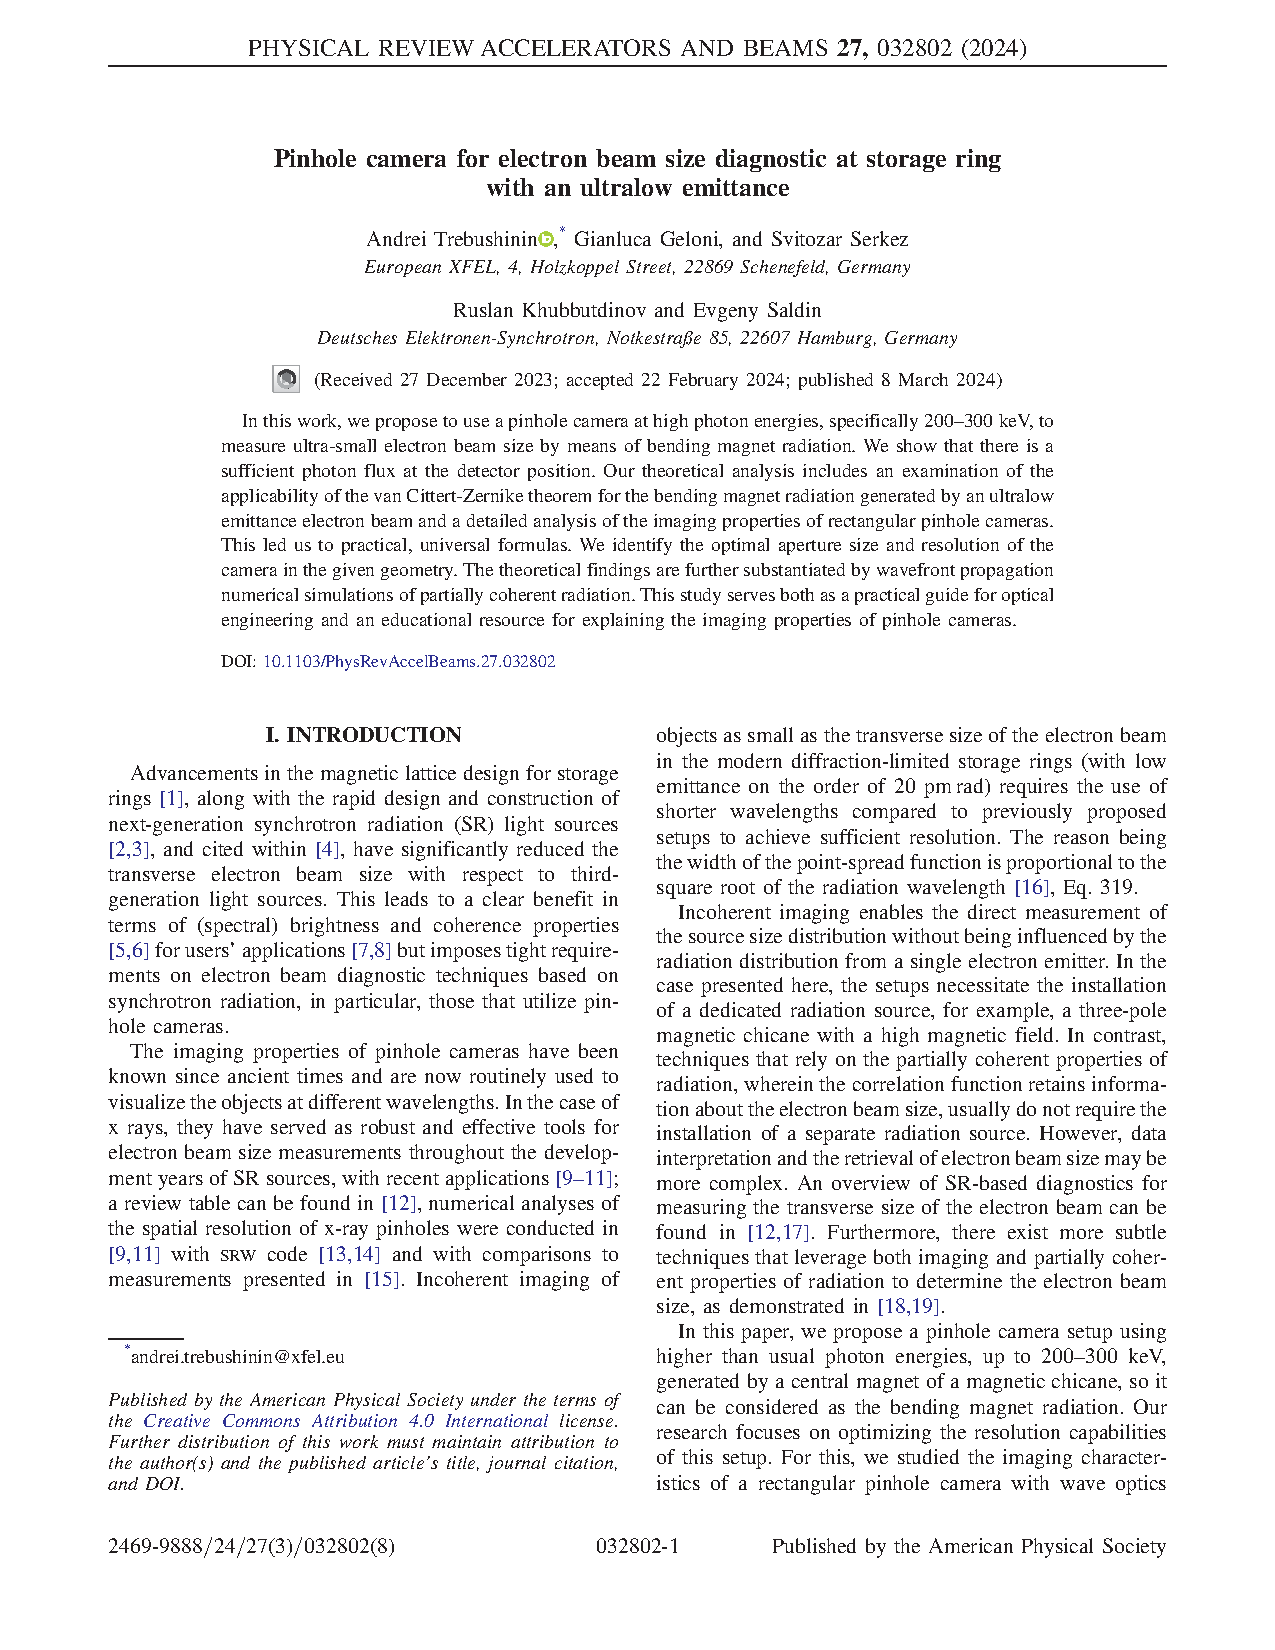
\includepdf[pages=-]{content/papers/pinhole.pdf}

\setcounter{mycounter}{2}
\section{Heuristic approach \Roman{mycounter}: quasi- homogeneous/stationary sources}
\label{Heuristic approach II: quasi- homogeneous/stationary sources}
    In the Section~\ref{sec:Heuristic approach: homogeneous/stationary source}, I have shown a method for simulating fully incoherent sources. In this section, I would like to extend these algorithms to account for finite source divergence. As will become clear from the derivation, confining the divergence of a source will inevitably result in an increased coherence length. Moreover, the resulting field will follow the correct correlation function.
    
    I take the previous Eq.~\ref{Eq:SERVAL0} and the make a Fourier transform of it to the inverce domain:
    \begin{align}
        \bar{\phi}(\vec{k}) = \mathcal{F} \big[ \sqrt{I(\vec{r})} \mathcal{N}(\vec{r})\big](\vec{k})
    \end{align}
    where Fourier transform is denoted as $\mathcal{F} \big[…\big]$ operator. Then I multiply this field by the effective radiation divergence at the source location $\hat{I}(\vec{k})$ and take inverse Fourier transform back the real space:
    \begin{align}
        \phi(\vec{r}) = \mathcal{F}^{-1} \bigg[ \sqrt{\hat{I}(\vec{k})} \mathcal{F} \big[ \sqrt{I(\vec{r})} \mathcal{N}(\vec{r})\big](\vec{k})\bigg](\vec{r}).
        \label{Eq:SERVAL1}
    \end{align}
    Again the hypothesis is that the field in Eq.~\ref{Eq:SERVAL1} follows correct correlation function. To check this I perform auto-correlation and write the integrals of the direct Fourier transform explicitly:
    \begin{align}
        \langle \phi(\vec{r}_1) \phi^*(\vec{r}_2) \rangle =  
        \mathcal{F}^{-1} \bigg[  \sqrt{\hat{I}(\vec{k}_1)\hat{I}(\vec{k}_2)} \iint \limits_{-\infty}^{\infty}  \sqrt{I(\vec{r}'_1)I(\vec{r}'_1)} \big \langle\mathcal{N}(\vec{r}'_1)\mathcal{N}(\vec{r}'_2) \big \rangle e^{i (\vec{r}'_1\vec{k}_1 - \vec{r}'_2\vec{k}_2)}d\vec{r}'_1 d\vec{r}'_2  \bigg](\vec{r}_1, \vec{r}_2),
    \end{align}
    where I bring the averaging sign under the integral sign and accounting for the noise property: $\langle \mathcal{N}(\vec{r}_1)\mathcal{N}^*(\vec{r}_2)\rangle = \delta(\vec{r}_2 - \vec{r}_1)$ I result in the following expression:
    \begin{align}
        \langle \phi(\vec{r}_1) \phi^*(\vec{r}_2) \rangle =  
        \mathcal{F}^{-1} \bigg[  \sqrt{\hat{I}(\vec{k}_1)\hat{I}(\vec{k}_2)}  \iint \limits_{-\infty}^{\infty}  \sqrt{I(\vec{r}'_1)I(\vec{r}'_1)} \delta(\vec{r}'_1 - \vec{r}'_2) e^{i (\vec{r}'_1\vec{k}_1 - \vec{r}'_2\vec{k}_2)}d\vec{r}'_1 d\vec{r}'_2 \bigg](\vec{r}_1, \vec{r}_2).
    \end{align}
    After this I integrate over $d\vec{r}_1$ accounting for the filtering property of Dirac delta function and obtain:
    \begin{align}
        \langle \phi(\vec{r}_1) \phi^*(\vec{r}_2) \rangle =  
        \mathcal{F}^{-1} \bigg[ \sqrt{\hat{I}(\vec{k}_1)\hat{I}(\vec{k}_2)} \int \limits_{-\infty}^{\infty}  I(\vec{r}') e^{i (\vec{r}'(\vec{k}_1 - \vec{k}_2)}d\vec{r}'  \bigg](\vec{r}_1, \vec{r}_2).
    \end{align}
    The explicitly written integral in this expression contains another integral that resembles one from the generalized van Cittert-Zernike theorem. So, changing this to $\hat{g}(\Delta \vec{k})$:
    \begin{align}
        \langle \phi(\vec{r}_1) \phi^*(\vec{r}_2) \rangle =  
        \iint \limits_{-\infty}^{\infty}  \sqrt{\hat{I}(\vec{k}_1)\hat{I}(\vec{k}_2)}\hat{g}(\Delta \vec{k}) e^{-i (\vec{r}_1\vec{k}_1 - \vec{r}_2\vec{k}_2)} d\vec{k}_1 d\vec{k}_2.
    \end{align}
    Then changing $\sqrt{\hat{I}(\vec{k}_1)\hat{I}(\vec{k}_2)}\hat{g}(\Delta \vec{k})$ by $\langle \hat{E}(\vec{k}_1) \hat{E}^{*}(\vec{k}_2) \rangle$ following the general definition of quasi-homogeneity in Eq.~\ref{Eq:quasi_homogeneous_source_weak}. Then, I result in the following expressions:
    \begin{align}
        \langle \phi(\vec{r}_1) \phi^*(\vec{r}_2) \rangle = \cr 
        = \iint \limits_{-\infty}^{\infty} \langle \hat{E}(\vec{k}_1) \hat{E}^{*}(\vec{k}_2) \rangle  e^{-i (\vec{r}_1\vec{k}_1 - \vec{r}_2\vec{k}_2)} d\vec{k}_1 d\vec{k}_2 = \cr
        = \bigg\langle \int \limits_{-\infty}^{\infty} \hat{E}(\vec{k}_1) e^{-i \vec{r}_1\vec{k}_1} d\vec{k}_1 \int \limits_{-\infty}^{\infty} \hat{E}^{*}(\vec{k}_2) e^{i \vec{r}_2\vec{k}_2} d\vec{k}_2 \bigg\rangle = \langle E(\vec{r}_1)E^{*}(\vec{r}_2) \rangle.
    \end{align}
    I have derived that the field $\phi(\vec{r})$ follows the same correlation function as the field $E(\vec{r})$. Since we are working with Gaussian random processes, higher-order correlation functions can be expressed in terms of the first-order correlation function.

    \rr{actually it would be very nice to show that power distribution follow negative exponent.}
    
    In Paper II, I discuss the implementation of this algorithm in the context of undulator radiation. It is important to note that the variables in the algorithm can be exchanged for longitudinal ones, yielding the same results. This equivalence highlights the mathematical similarity between the van Cittert-Zernike theorem and the Wiener-Khinchin theorem. For instance, this algorithm can be used to simulate the longitudinal domain of chirp-free SASE radiation from a free-electron laser (FEL).

    \rr{again write some more}
    
\newpage    
\setcounter{mycounter}{2} % Set the counter to 1
\section{Paper \Roman{mycounter}}

    In the paper by A. Trebushinin, G. Geloni, Y. Rakshun, and S. Serkez, Gaussian Random Field Generator for Simulating Partially Coherent Undulator Radiation, Optica 9, 842 (2022),
    we introduced a computationally efficient algorithm to simulate partially coherent synchrotron radiation fields from undulators, specifically tailored for applications in modern synchrotron radiation sources with low electron beam emittance. This simulation addresses the stochastic nature of radiation fields that arise from shot noise in electron beams, an aspect often simplified and discarded in synchrotron radiation simulations.
    
    The proposed method, referred to as the Synchrotron Emission Rapid eVALuator (SERVAL), utilizes Gaussian random fields to generate statistical realizations of the radiation field at a given frequency. This technique allows to shape a complex amplitude by constraining complex Gaussian noise by the effective size and divergence of the radiation field as have been described in Sec.~\ref{Heuristic approach II: quasi- homogeneous/stationary sources}. This algorithm significantly speeds up the calculations compared to traditional Monte Carlo-like approaches. As a result, we obtain undulator radiation fields that encompass all coherent modes at once if we think of the result in terms of coherent mode decomposition methods.
    
    We provide a detailed theoretical background on the statistical properties of undulator radiation, highlighting the intrinsic stochastic structure due to the random distribution of electrons within the beam. They illustrate how our approach is consistent with established theoretical frameworks and offers computational algorithms. The method has been validated against other simulation approaches, demonstrating its effectiveness in capturing the statistical properties of synchrotron radiation.
    
    Practically, SERVAL capabilities are demonstrated through simulations that involve typical components of synchrotron beamlines, such as focusing systems. These demonstrations show how the method can be integrated into existing simulation frameworks like Ocelot~\cite{ocelot-collab_ocelot_2017} for comprehensive start-to-end modeling of radiation at synchrotron facilities. In summary, this paper presents an advancement in the simulation of synchrotron radiation, offering a fast and accurate method to model the partially coherent radiation produced by undulators. We believe that this approach not only enhances the design and optimization of synchrotron light sources but also serves as an educational tool for understanding complex radiation phenomena.

\includepdf[pages=-]{content/papers/SERVAL.pdf}
\section{Coherence properties of SASE FEL radiation}
    In this section, I will briefly discuss the coherence properties of SASE FEL. Comprehensive presentations on the statistical properties of SASE FEL can be found in pioneering works~\cite{saldin_statistical_1998} and in textbooks on FEL physics. Here, I will outline the fundamental aspects needed for the further development of the SERVAL algorithm. I will focus on the longitudinal coherence properties of SASE radiation, assuming that the radiation is fully coherent transversely. I will revisit this point at the conclusion of this chapter.

    \rr{this difficult to read, improve this}
    
    The theory previously outlined in this thesis encapsulates the statistical properties of Gaussian processes and is applicable to more complex processes like SASE, albeit with some limitations. SASE amplification, despite its laser-like name, starts from usual synchrotron radiation. Up to the moment of saturation\footnote{The term refers to the phase where there is an exponential gain in the power of radiation.}, Gaussian statistics are preserved. This regime of operation is called the linear regime, which refers to the exponential gain in the power of radiation. The term "linear" is used in reference to electric circuits amplifiers. Only after reaching saturation the radiation statistics start to deviate from Gaussian statistics, as described in~\cite{saldin_statistical_1998}. Therefore, for developing SERVAL, it means that up to the moment of saturation, one can apply SERVAL-like algorithms. For illustration, I plot the evolution of the SASE process in Fig.~\ref{Fig:evo_spikes} in addition to this, a more detailed explanation on SASE process within this thesis can be found in Paper IV,~\cite{trebushinin_experimental_2023}.
    \begin{figure*}[h!]
    	\centering
        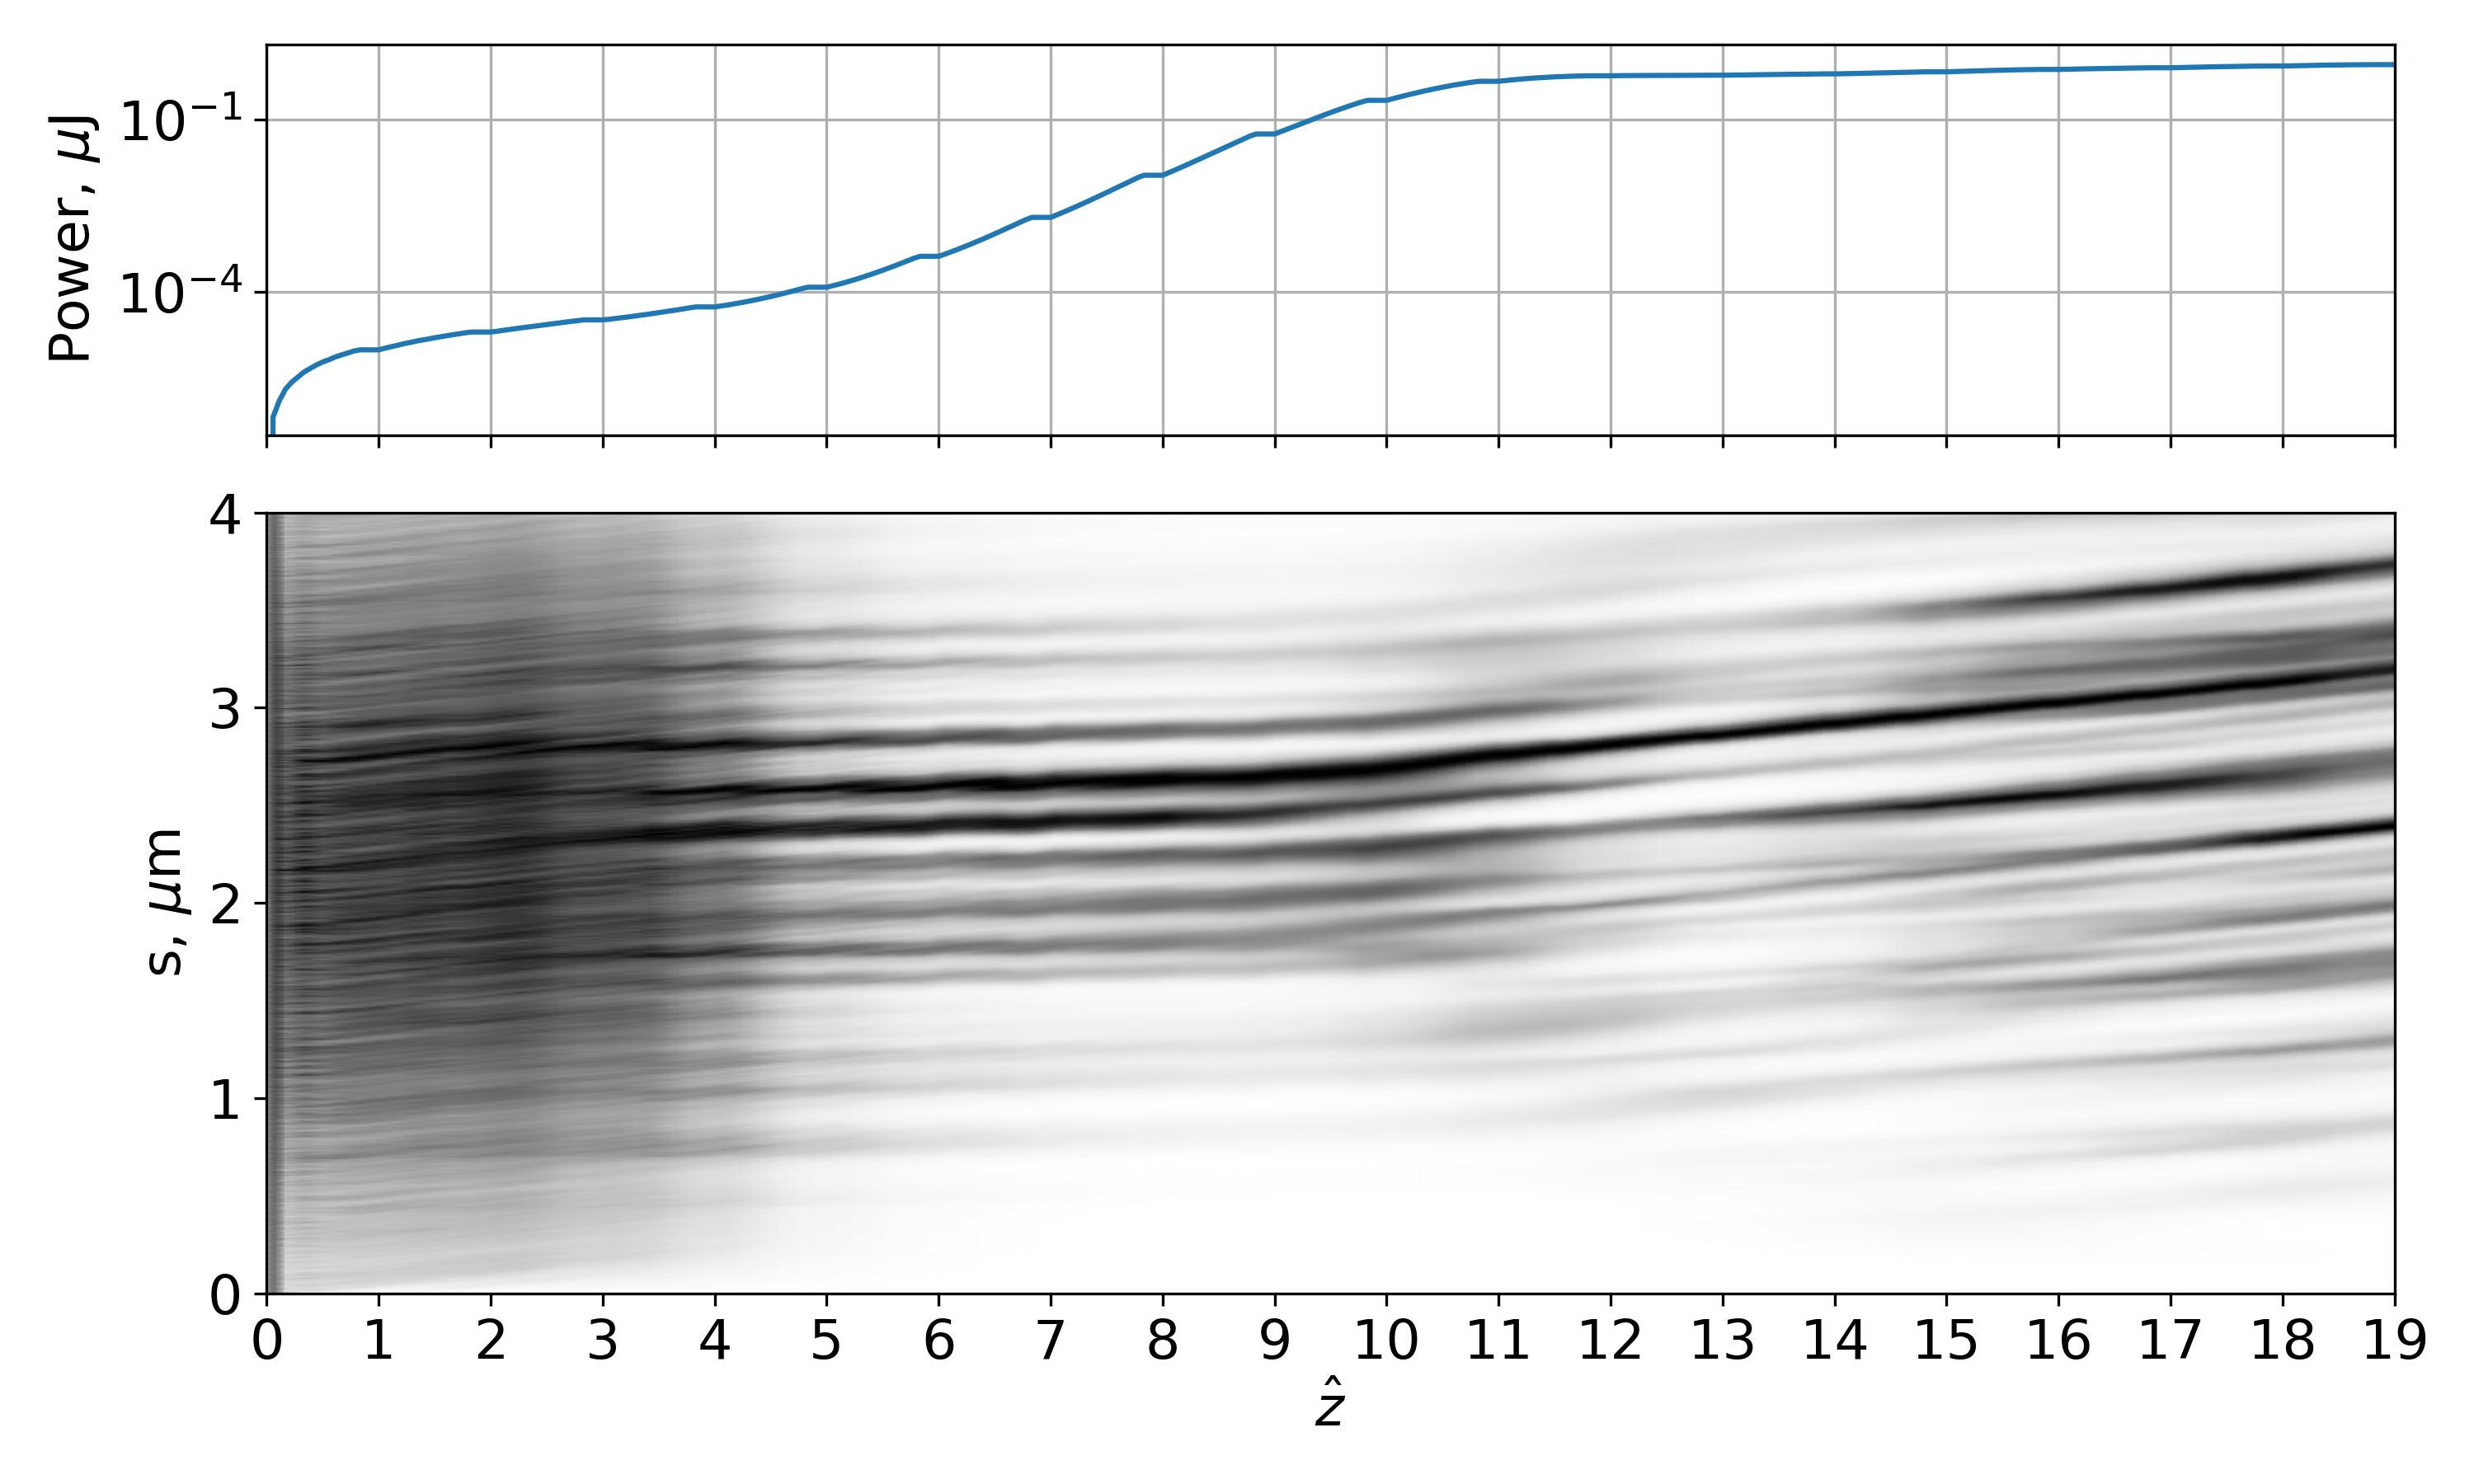
\includegraphics[width=0.95\linewidth]{content/images/4_FEL_Theory/evo_spikes.png}
    \captionsetup{justification=centering}
        \caption{SASE lasing process: Radiation starts from shot noise and is steadily amplified exponentially until reaching saturation around $\hat{z} = 10$, after which the radiation power grows nearly linearly.}
        \label{Fig:evo_spikes}
    \end{figure*}
    
    Transversely, radiation undergoes a mode selection process and rapidly acquires almost full transverse coherence. I illustrate this in Fig.~\ref{Fig:transverse_modes}:
    \begin{figure*}[h!]
    	\centering
        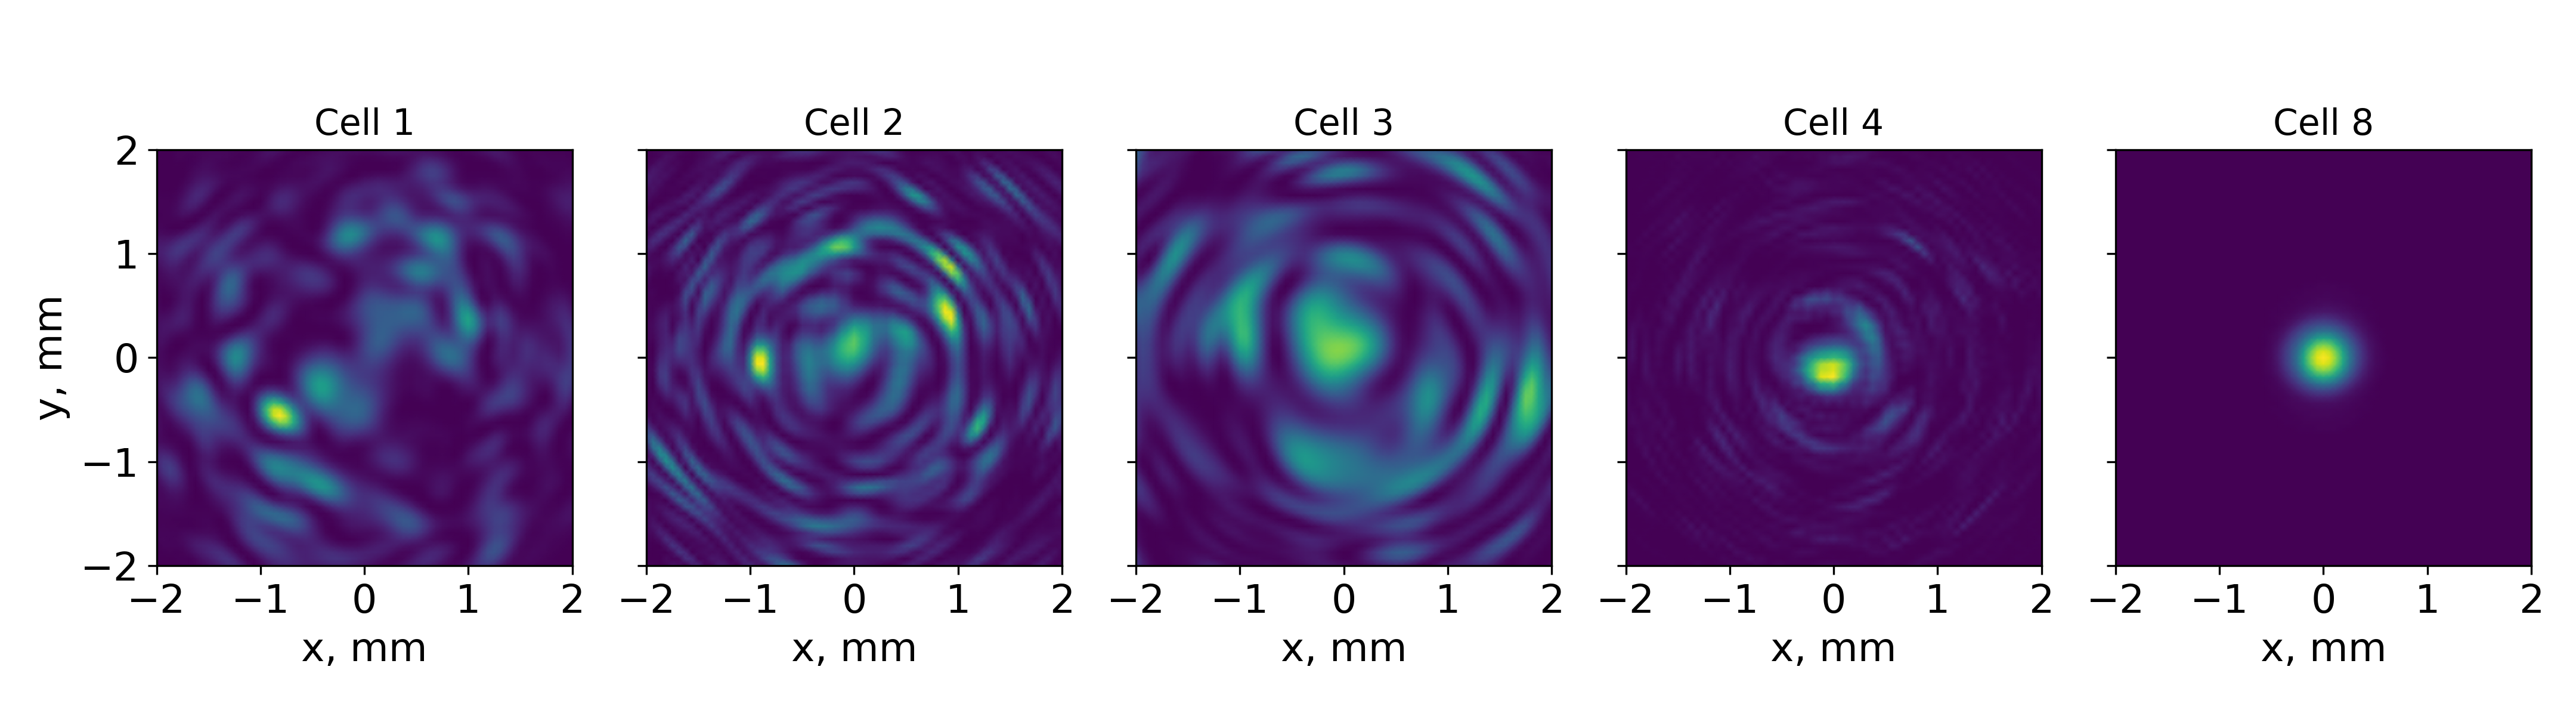
\includegraphics[width=0.99\linewidth]{content/images/4_FEL_Theory/transverse_modes.png}
        \captionsetup{justification=centering}
        \caption{Transverse intensity distribution of monochromatized radiation view in the far zone from the number of cell labeled on top of sub figure.}
        \label{Fig:transverse_modes}
    \end{figure*} 
    From here on, I assume that SASE radiation is in a transversely coherent state, and I focus on describing the longitudinal domain of the SASE radiation, as it is of the most interest for practical cases.

    Radiation properties in the longitudinal (time-frequency) domain heavily depend on the energy chirp in the electron beam. It can be easily shown with the undulator resonance condition that the energy chirp of the electron beam relates to the radiation frequency as follows:
    \begin{align}
        \omega(t) = \frac{2 \gamma^2(t)k_w c}{1 + K^2/2},
    \end{align}
    where $\gamma(t) = \gamma_0 + \gamma_n(t)$. Normally the value of energy variation $\gamma_n(t)$ is so small (i.e. $\gamma_n(t)/\gamma_0 \ll 1$) that one can expand $\gamma^2(t)$ and obtain the following expression:
    \begin{align}
        \omega(t) = \frac{2\gamma_0^2k_w c}{1 + K^2/2}\bigg(1 + 2\frac{\gamma_n(t)}{\gamma_0}\bigg) 
    \end{align}
    As one can see here, in the first approximation, SASE radiation's instantaneous frequency replicates the chirp in the electron beam. Now, it is time to examine the phase space of such radiation.
    
    One way to represent the structure of the radiation phase is through the Wigner distribution, which I define as follows:
    \begin{align}
        \mathcal{W}(\bar{t}, \bar{\omega}) = \int \limits_{-\infty}^{\infty} \Tilde{\Gamma}(\bar{\omega}, \Delta \omega) e^{-i\Delta \omega \bar{t}}d(\Delta \omega)
    \end{align}

    Having this, one can represent the radiation distribution in the space of the time-domain (longitudinal coordinate along the beam) and frequency (photon energy). Moreover, one can represent a single statistical realization in terms of the Wigner function distribution. This can be done based on the fact that the averaging operation for $\Tilde{\Gamma}(\bar{\omega}, \Delta \omega)$ can be taken out of the integral, i.e., taking the integral and averaging can be exchanged in order. In this way, a Wigner function of a single realization makes sense, as well as averaging single-shot Wigner functions to obtain an averaged one.
    
    In Fig.~\ref{Fig:ROSA_linear_chirp}, I present such a Wigner function from a single realization of SASE radiation from a linearly chirped electron beam. With this figure, I introduce important concepts such as instantaneous bandwidth, instantaneous frequency, group delay, and group duration, which are outlined in Fig.~\ref{Fig:ROSA_linear_chirp} and are hopefully self-explanatory. 
    \begin{figure}[h!]
    	\centering
        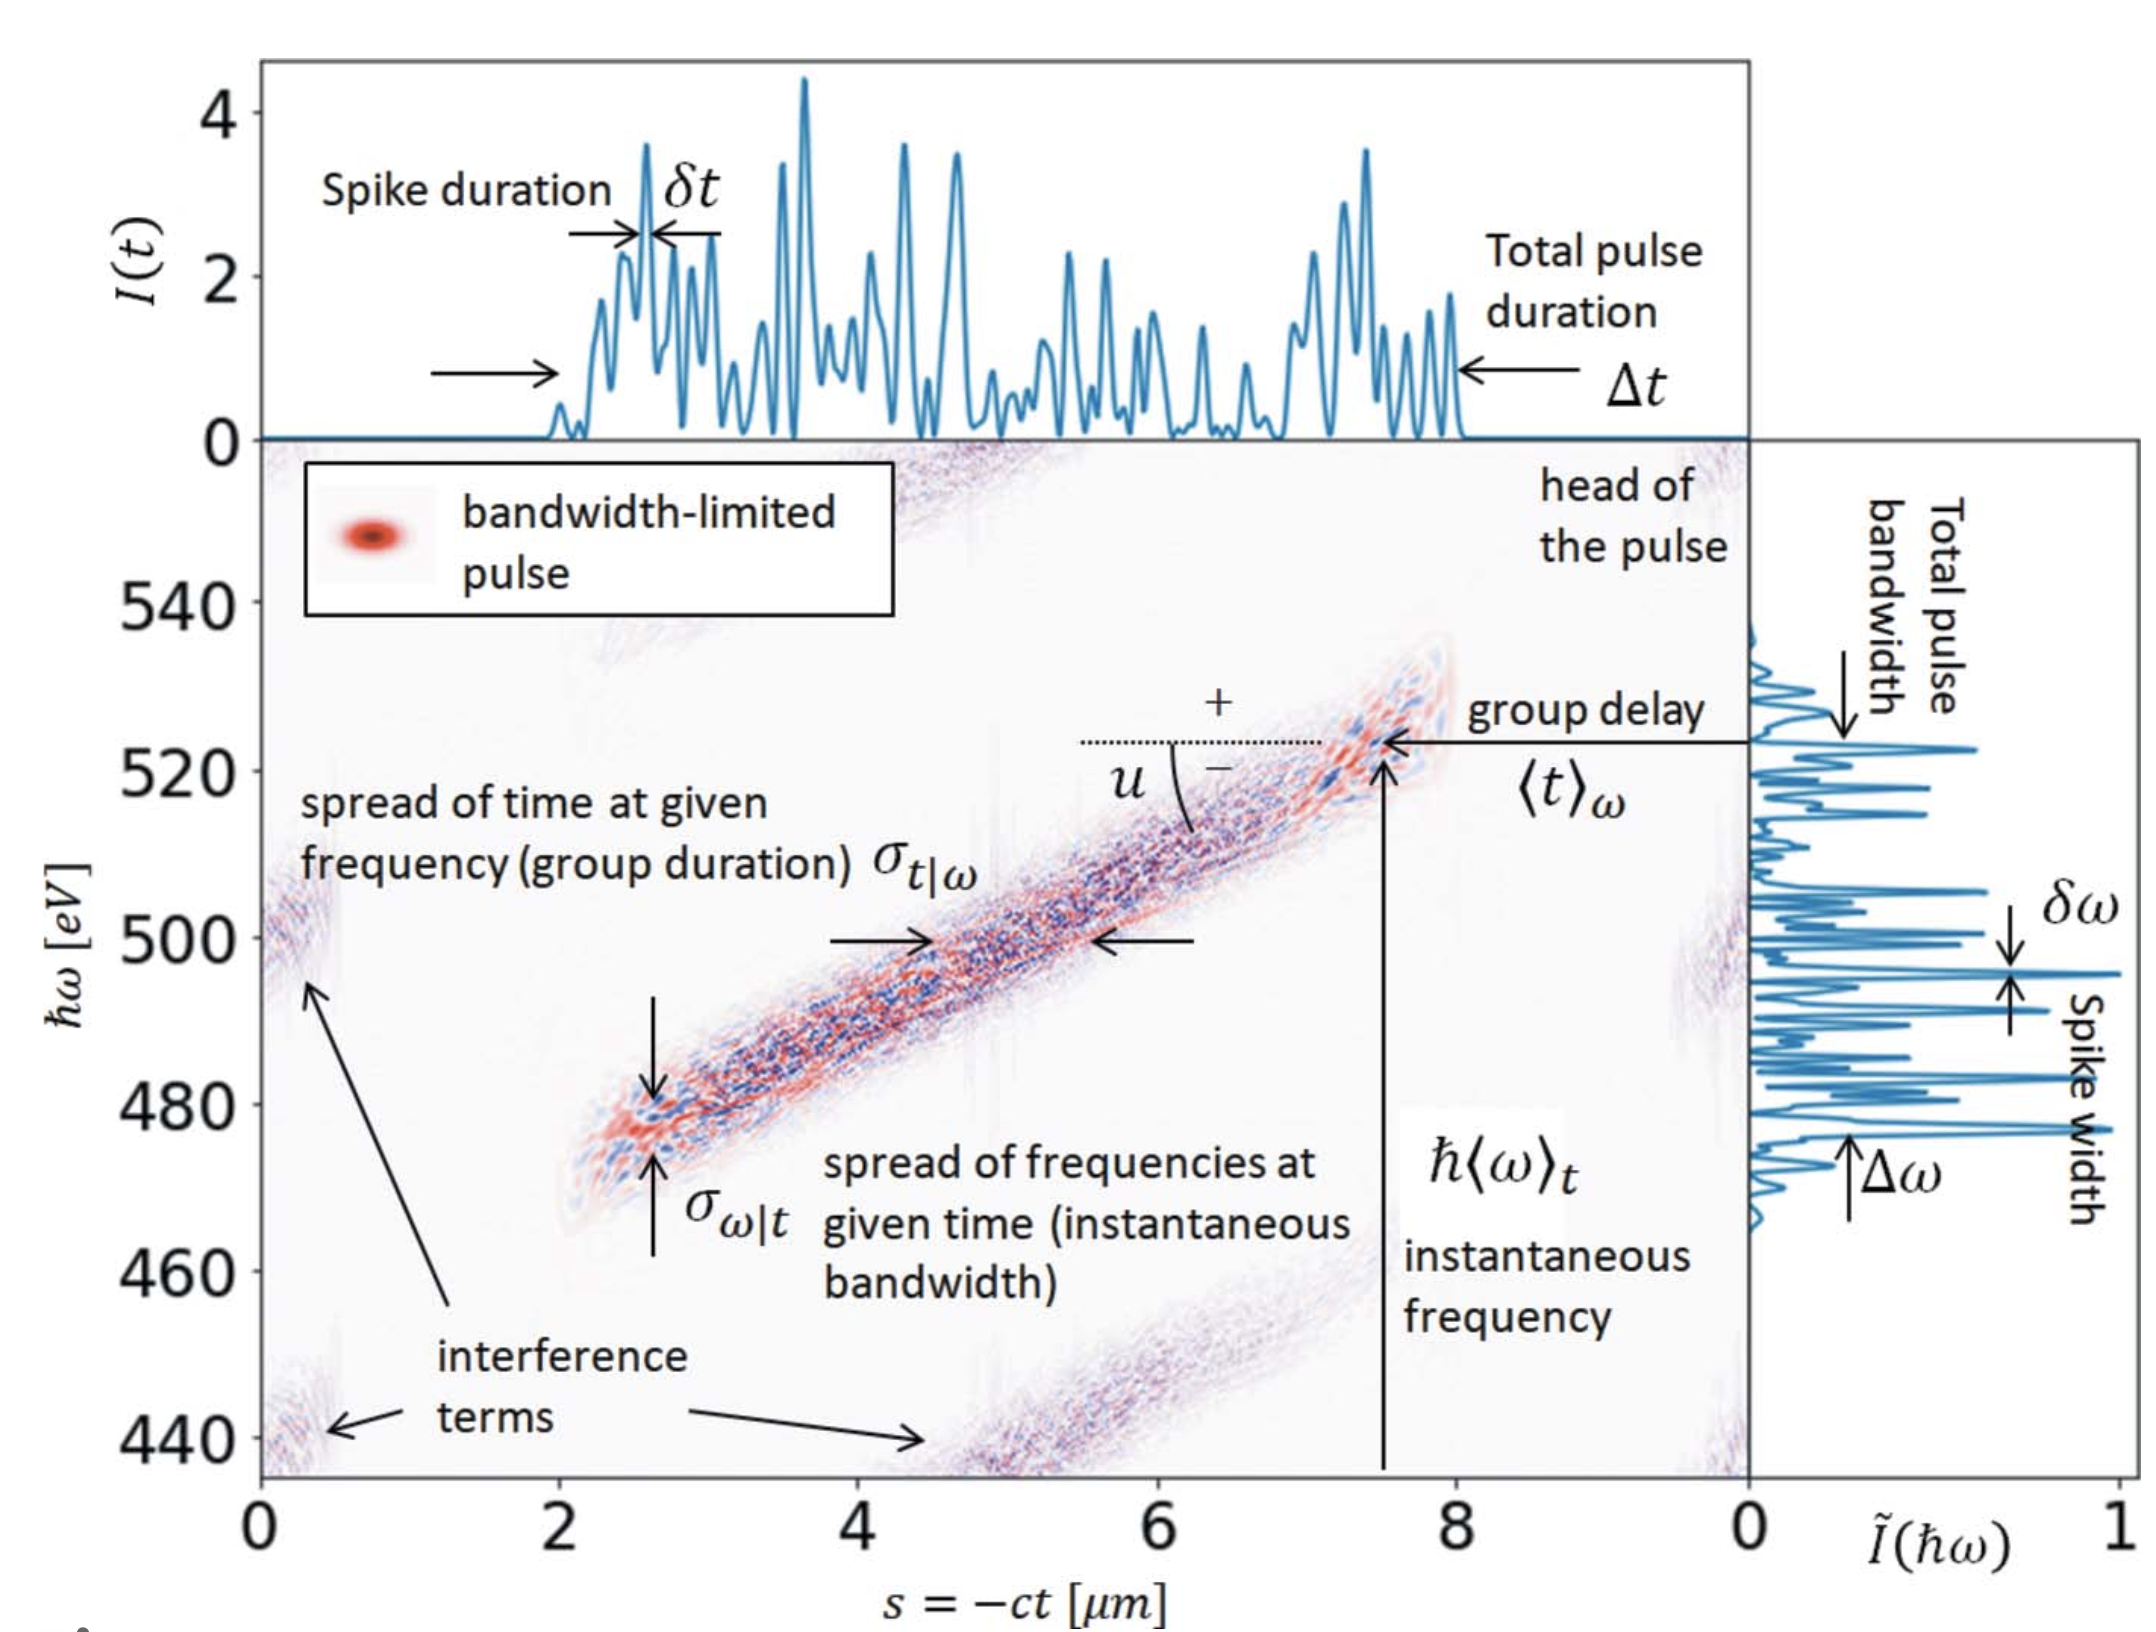
\includegraphics[width=0.75\linewidth]{content/images/4_FEL_Theory/ROSA_linear_chirp.png}
        \captionsetup{justification=centering}
        \caption{\textbf{Adopted from \cite{serkez_wigner_2021}} The European XFEL 100 pC electron beam with a non-linear energy chirp produces SASE radiation with different durations at different photon energies. Note the bifurcation in Wigner distribution above 499 eV. Analysis based on 1000 simulated SASE spectra.}
        \label{Fig:ROSA_linear_chirp}
    \end{figure} 
    In real experiments at facilities such as the European XFEL, electron beams often exhibit nonlinear frequency chirps~\rr{cite}. A simulation of one such example is presented in Fig.~\ref{Fig:ROSA_sim}. Simulating these distributions aims to reproduce results from the real experiment and validate the ROSA algorithms~\cite{serkez_wigner_2021}.
    \begin{figure}[h!]
    	\centering
        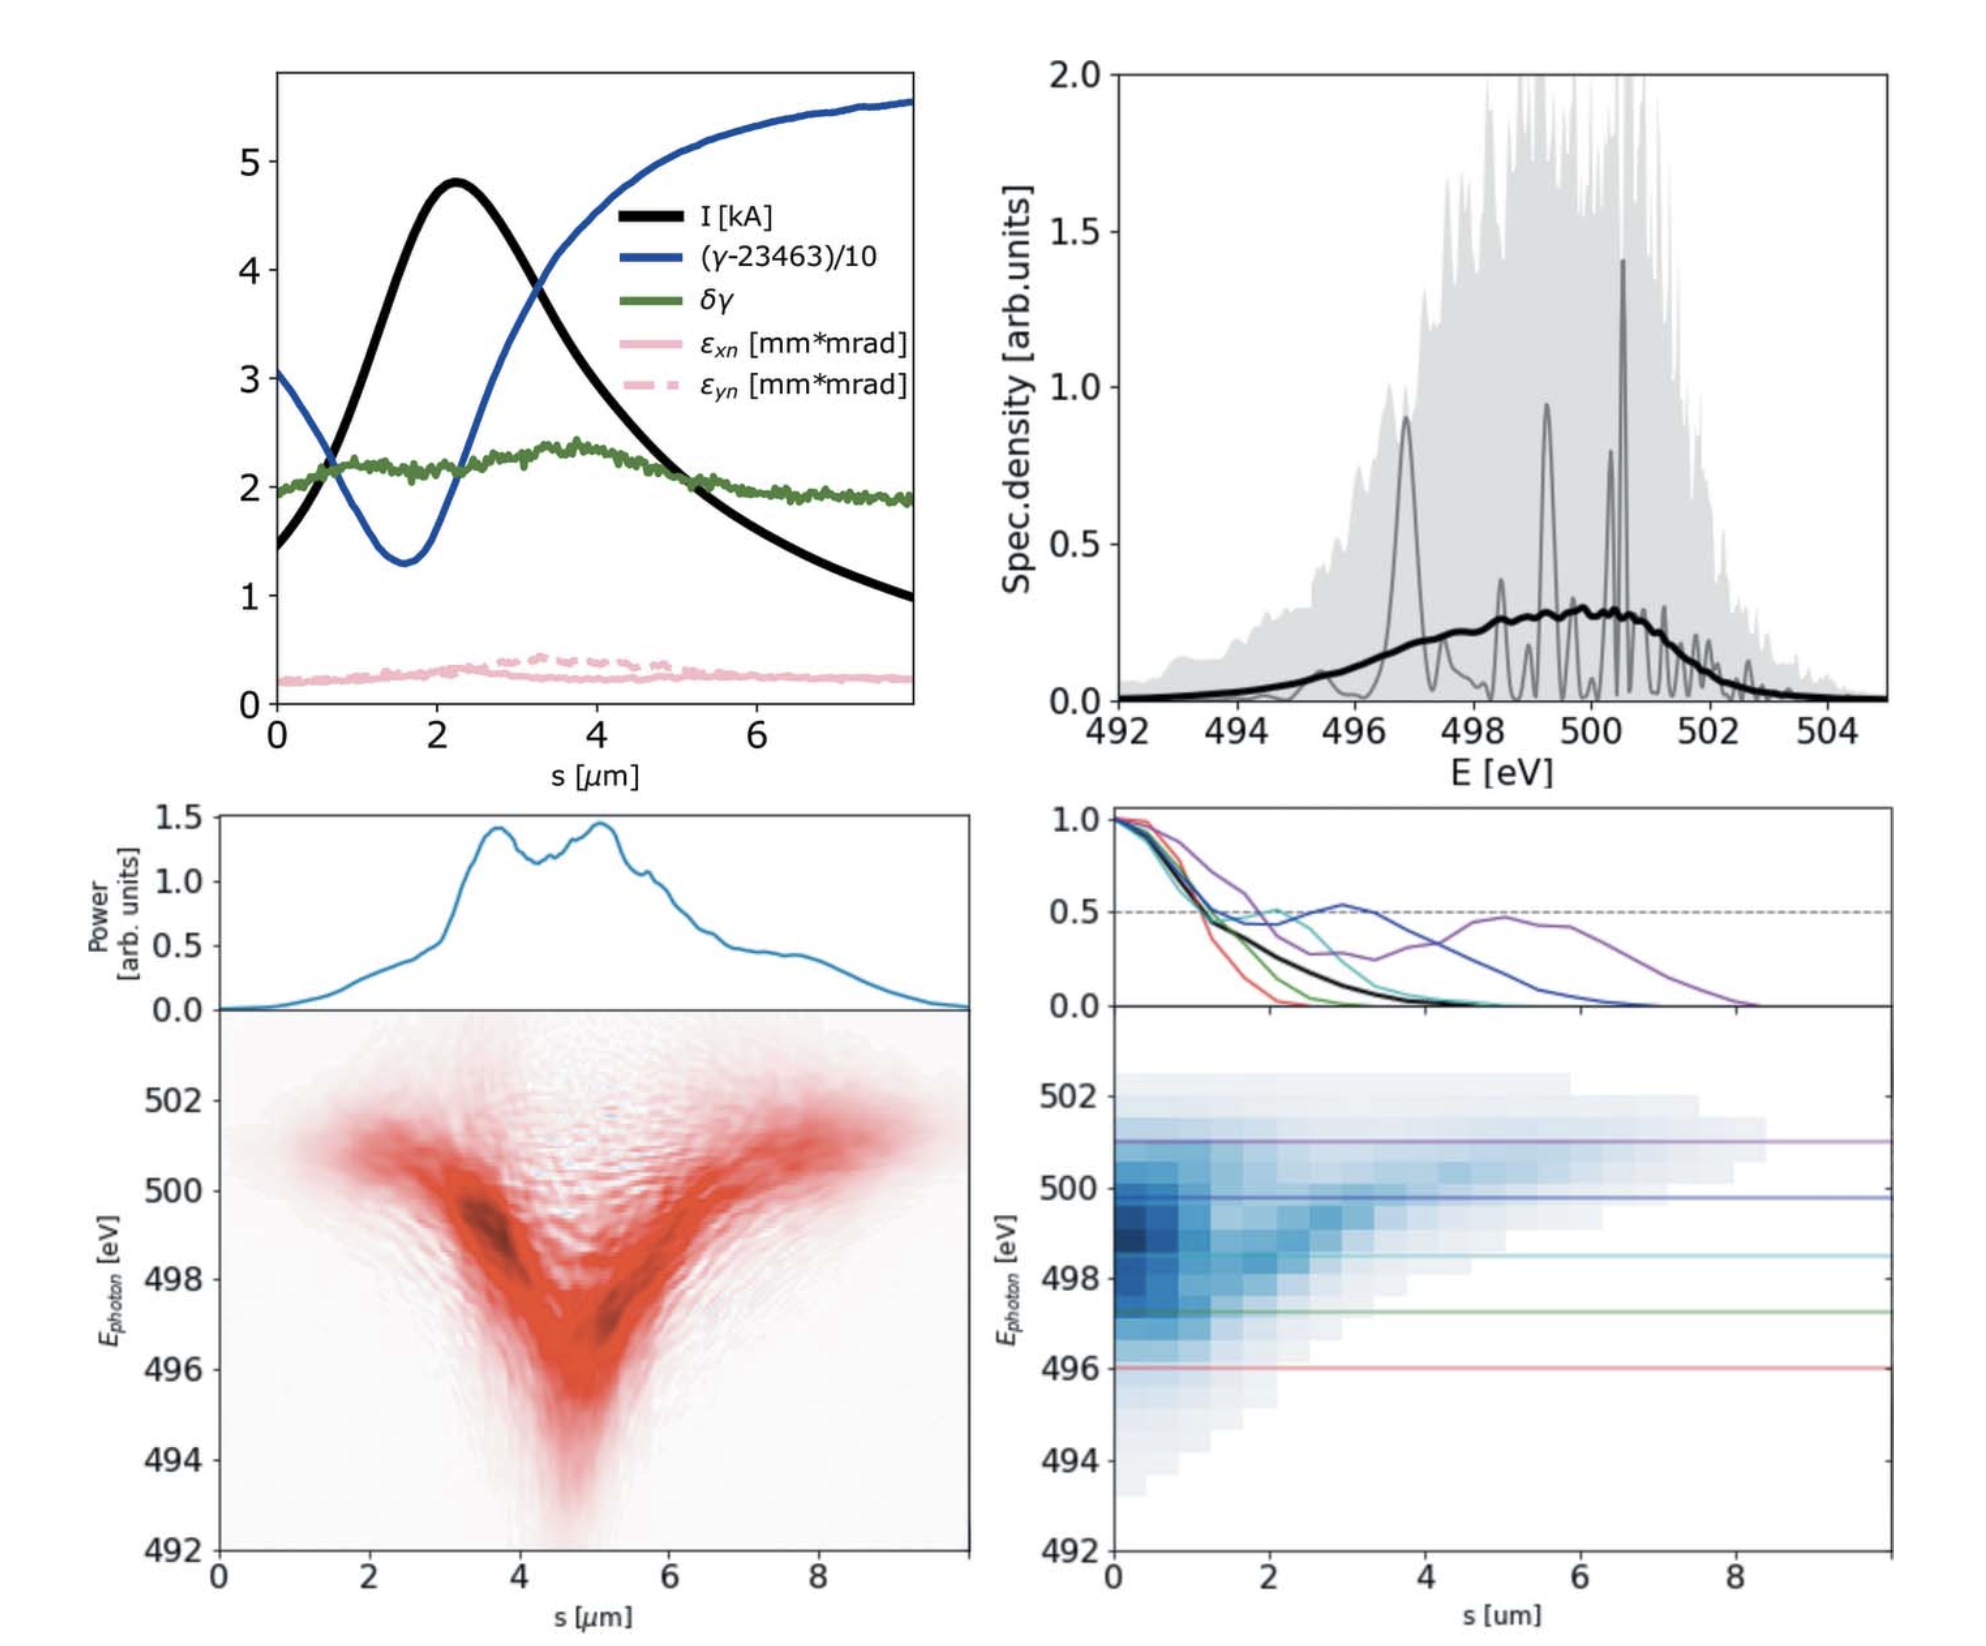
\includegraphics[width=0.75
        \linewidth]{content/images/4_FEL_Theory/ROSA_sim.png}
        \captionsetup{justification=centering}
        \caption{\textbf{Adopted from \cite{serkez_wigner_2021}}}
        \label{Fig:ROSA_sim}
    \end{figure} 
    The next goal for developing the SERVAL algorithm is to enable it to account for these kinds of frequency chirps or, more generally, arbitrary Wigner function distributions of the radiation. The results of this activity are presented in the subsequent section and in Paper IV.

\setcounter{mycounter}{3}
\section{Heuristic approach \Roman{mycounter}: non- homogeneous / stationary sources}

    One may notice that for a source that can be represented $\Tilde{\Gamma}(\omega, \Delta \omega) = f_{\omega}(\Delta \omega)\bar{I}(\bar{\omega})$ it is possible to take the intensity out under the integral sign, so Wigner function $\mathcal{W}(t, \omega)$ can be written as the following:
    \begin{align}
        \mathcal{W}(\bar{t}, \bar{\omega}) = \bar{I}(\bar{\omega}) \int \limits_{-\infty}^{\infty} f_{\omega}(\Delta \omega) e^{-i\Delta \omega \bar{t}}d(\Delta \omega) = \bar{I}(\bar{\omega}) I(\bar{t}).
    \end{align}
    Looking at this expression and \textit{mentally}\footnote{I mention here again that throughout this chapter, I present the algorithms in different pairs of domains — spatial-inverse spatial and time-frequency domains. This is justified by the fact that the van Cittert-Zernike theorem for the transverse domain and the Wiener-Khinchin theorem for the longitudinal domain are similar relations, i.e., both are based on Fourier transforms. Thus, I use the same algorithms for these pairs of domains almost without changes.} changing the variables to transverse ones, it is clear that in the previous version of SERVAL in Eq.~\ref{Eq:SERVAL1}, I implicitly used the factorized Wigner function.
    
    Now instead of factorising the Wigner function, I write it as it is under the first integral:
    \begin{align}
    	\phi(\bar{\omega}) = \int \limits_{-\infty}^{\infty} \sqrt{\mathcal{W}(\bar{\omega}, \bar{t})} \mathcal{N}(\bar{t}) e^{i \bar{\omega} \bar{t}} d\bar{t}.
    	\label{Eq:Field_Wigner}
    \end{align}
    My hypothesis is the following: Eq.~\ref{Eq:Field_Wigner} can indeed represent a real field that has the correlation function $\Tilde{\Gamma}(\omega, \Delta \omega)$. This I will study the following Paper III.
    
\newpage    
\setcounter{mycounter}{3} % Set the counter to 1
\section{Paper \Roman{mycounter}}
    
    In the paper A. Trebushinin, G. Geloni, and S. Serkez, Algorithm for modeling partially coherent radiation with an arbitrary Wigner function, we introduce an upgraded algorithm compared to one presented in~\cite{trebushinin_gaussian_2022}. This approach utilizes a Wigner function distribution to accurately model the stochastic properties of radiation fields, which is particularly relevant for advanced radiation sources like synchrotrons and free-electron lasers (FELs).
    
    The algorithm builds on the concept of simulating Gaussian random fields, where noise is generated and then constrained by the effective support in both Fourier domain weather it is time -- frequency one or spatial -- inverse spatial. This method is computationally efficient and allows for the propagation of the simulated field through various optical elements. We verified that the simulated fields adhere to the correct statistical descriptions by comparing ensemble-averaged intensities and correlation functions against theoretical predictions and numerical results. The paper elaborates on several key applications, including simulations of double-slit experiments and SASE radiation from FELs. These examples demonstrate the versatility of the algorithm in handling different types of radiation sources, including those with complex temporal and spatial coherence properties as SASE radiation with different frequency chirps.
    
    We also discuss potential extensions of the algorithm, suggesting its applicability to non-Gaussian sources and more complex spatial-temporal coherence scenarios. We argue on the algorithm's flexibility and computational efficiency make it a potent tool for both research and educational purposes in the field of physical and statistical optics. Overall, the paper provides a comprehensive framework for simulating partially coherent radiation, with significant implications for the design and analysis of optical systems and experiments in modern synchrotron and FEL facilities.
    
\includepdf[pages=-]{content/papers/SERVAL2.pdf}


\newpage    
\setcounter{mycounter}{4} % Set the counter to 1
\section{Paper \Roman{mycounter}}
    In the following paper I will present a special mode of SASE FEL operation, demonstrating that the resulting radiation does not adhere to Gaussian statistics. With this example, I aim to illustrate that the application of SERVAL algorithms should always be done thoughtfully, based on the specific case under study. For instance, when it was not possible to use SERVAL, I had to perform simulations using the Genesis 1.3 code.
    
    In the paper A. Trebushinin, G. Geloni, S. Serkez, G. Mercurio, N. Gerasimova, T. Maltezopoulos, M. Guetg, and E. Schneidmiller, Experimental Demonstration of Attoseconds-at-Harmonics at the SASE3 Undulator of the European XFEL, Photonics 10, 2 (2023), we present an experiment generating sub-femtosecond pulses using the 'attosecond-at-harmonic' method at Free Electron Lasers (FELs). The research, conducted at the European XFEL's SASE3 undulator, demonstrated a method to produce short pulses through harmonic conversion, specifically targeting the fourth harmonic.

    The experimental setup involved a two-stage process. In the first stage, the undulator amplified the electron bunching at both the fundamental frequency and higher harmonics. In the second stage, the SASE3 undulator, tuned specifically to the fourth harmonic, further amplified these pulses to achieve shorter durations. Statistically, not all pulses were single-spike events, but we identified that depending on the experimental conditions, 3\% to 13\% of the generated pulses were single-spike events. In the paper, we report the creation of pulses with a lower estimated duration of 650 attoseconds.
    
    The technique described, referred to as the 'attoseconds-at-harmonics' method, utilizes minimal hardware modifications, relying only on variable gap undulator cells to achieve the desired harmonic amplification. This method proved to be versatile in settings with limited hardware at a beamline, offering a way to generate short X-ray pulses suitable for probing fast dynamics in materials science, chemistry, and other fields.
    
    This paper outlines not only the experimental setup and results but also discusses the theoretical background, specifically the process of harmonic conversion. The statistics of this radiation are non-Gaussian due to the nonlinear conversion process, as shown in the paper. Interpreting the spectral width to estimate the resulting pulse duration is complicated because there is no direct relationship between the first-order correlation function and higher-order ones usually applied for pulse duration estimation. In this paper, we developed a simulation-based method to provide a correction factor that helped us resulted in a lower estimate of the pulse duration.
    
\includepdf[pages=-]{content/papers/attoharm.pdf}

\section{Conclusion}

    The content of this chapter is intended to enhance the results of the presented papers and vice versa. The chapter is supported by the necessary theoretical background, including an introduction to types of random processes and a discussion of important classes of sources such as stationary and ergodic sources. I then introduced the concept of Gaussian statistics for random processes, which significantly simplifies the analysis of random processes by linking higher-order correlation functions with the first-order one. Following this, I explored concepts such as quasi-stationarity and homogeneity, highlighting their mathematical similarities. Concluding the theoretical part, I outlined coherence theory for synchrotron radiation sources and free-electron lasers.

    \rr{It sounds sketchy, work on this more}
    
    The goal of this chapter is to present three algorithms for simulating fully incoherent fields, partially coherent fields, and partially coherent fields with arbitrary Wigner function distributions. These algorithms replicate  random fields by generating complex Gaussian noise and then constraining this noise with appropriate mathematical supports. For fully incoherent sources, the support is simply the random source intensity distribution. For partially coherent sources, this support is supplemented by the source's effective divergence in the inverse space domain. These approaches assume that the radiation phase space is factorized. However, the algorithm can be extended to simulate fields with arbitrary phase space distributions using the Wigner function. All three algorithms have practical applications, such as simulating bending magnet radiation, undulator radiation, and FEL SASE radiation in the linear regime. Additionally, I provided an interesting example of simulating the original Young's double slit experiment using one of the versions of the code. I have endeavored to explain not only the practical advancements of these algorithms but also their limitations, which are crucial to consider when simulating complex systems. For example, I mentioned a method that could potentially extend the applicability of these algorithms to non-Gaussian statistics, which could be a subject for further study beyond the scope of this thesis. In conclusion, I hope that the algorithms presented here will serve as valuable tools for optical simulations. Meanwhile, in the next chapter, I will present the result of the experiments for measuring electron beam size at hard X-ray beamlies of European XFEL where SERVAL played very important role at the stage of numerical simulations.
